\documentclass[preprint, 12pt, authoryear]{elsarticle}
\pdfoutput=1
\usepackage{etoolbox}
%\renewcommand*{\today}{August 29, 2018}
\patchcmd{\MaketitleBox}{\footnotesize\itshape\elsaddress\par\vskip36pt}{\footnotesize\itshape\elsaddress\par\parbox[b][36pt]{\linewidth}{\vfill\hfill\textnormal{\today}\hfill\null\vfill}}{}{}%
\patchcmd{\pprintMaketitle}{\footnotesize\itshape\elsaddress\par\vskip36pt}{\footnotesize\itshape\elsaddress\par\parbox[b][36pt]{\linewidth}{\vfill\hfill\textnormal{\today}\hfill\null\vfill}}{}{}%

\usepackage{eurosym} 
\usepackage{gensymb}
\usepackage{makecell}
\usepackage{subcaption}
\usepackage{url}
\usepackage{breakurl}
\def\UrlBreaks{\do\/\do-}

\usepackage[version=4]{mhchem} 
\usepackage{amsmath} 
\usepackage{amsfonts}
\usepackage{amssymb}
\usepackage{graphicx}

\usepackage{multibib}
\newcites{sec}{Bibliography} 

%\bibliographystyle{elsarticle-harv}

\makeatletter
\def\ps@pprintTitle{%
 \let\@oddhead\@empty
 \let\@evenhead\@empty
 \def\@oddfoot{}%
 \let\@evenfoot\@oddfoot}
\makeatother

\begin{document}
\begin{frontmatter}
\title{District heating systems under high \ce{CO2} emission prices: the role of the pass-through from emission cost to electricity prices}

\author[1,2]{Sebastian Wehrle\corref{cor1}}
\ead{sebastian.wehrle@boku.ac.at}

\author[1]{Johannes Schmidt}
\ead{johannes.schmidt@boku.ac.at}

\author[1]{Olga Turkovska}
\ead{olga.turkovska@boku.ac.at}

\cortext[cor1]{Corresponding author}

\address[1]{Institute for Sustainable Economic Development, University of Natural Resources and Life Sciences, Feistmantelstrasse 4, 1180 Vienna, Austria}

\address[2]{Wiener Netze GmbH, Erdbergstrasse 236, 1110 Vienna, Austria}

\begin{abstract}
In spite of recent increases, carbon prices in the European emission trading system are still below levels considered to be consistent with the goals of the Paris Agreement \citep[e.g.][]{Parry2018, OECD2018}.
The cost of \ce{CO2} emissions affects, inter alia, integrated district heating systems that use a variety of emission intense heat generation technologies. 
We study the effect of high carbon prices on district heating systems, operating within the current and a prospective future German electricity system.
%In addition, we examine how district heating system fare under a prospective further expansion of renewable power generation and an intended coal phase out.
Therefore, we (i) develop a simplified analytical framework to analyse optimal decisions of a district heating operator, and (ii) investigate the market-wide effects of increasing emission prices, in particular the pass-through from emission costs to electricity prices.
Using MEDEA, a numerical model of the power market in the German bidding area, we estimate a pass-through from \ce{CO2} emission prices to power prices between $0.82$ and $0.64$ as of 2017, depending on the absolute emission price level.
This suffices to improve the profitability of  natural gas-fired district heating systems of at least moderate efficiency under rising carbon prices. 
However, the emission cost pass-through is set to decline markedly in prospective electricity systems, rendering this a short-term opportunity.
\end{abstract}

\begin{keyword}
electricity markets \sep pass-through \sep carbon pricing \sep district heating
\JEL L94 \sep Q41 \sep C61
\end{keyword}
\end{frontmatter}
\newpage

\section{Introduction} \label{intro}
Combined heat and power (CHP) units produced $124$ TWh of electricity in 2017, accounting for $20.0\%$ of total German electricity generation \citep{AGEB2018a}. 
The CHP heat is used in industrial processes or for space heating through heat grids. In Germany, such district heating grids are found in virtually all major urban areas. 
In consequence, Germany is by far the largest consumer of district heat in Europe, with sales of $121.4$ TWh ($8.3\%$ of final heating demand) in 2017 \citep{AGEB2018b}. 
However, not all sold district heat is generated in natural gas or coal-fired CHP plants, as typical district heating systems rely on a broader portfolio of technologies. 
Many systems include waste incineration units and most use boilers to supply heat in times of peak load. 
Recently, district heating system operators also seek to include low-emission heat sources such as geothermal, solar thermal, biomass, or waste heat from commercial and industrial activities.

District heating systems are typically vertically integrated, with municipalities or federal states either holding majority stakes in district heating systems (e.g. in Cologne, Stuttgart, Frankfurt am Main, D\"usseldorf, Dortmund) or fully owning district heating systems in their district (e.g. Munich).\footnote{In Hamburg, the federal state currently holds a minority stake in the district heating system and is set to regain full control in 2019, while Berlin seeks to regain control over the district heating system, which was privatized in 2001. }
Against this backdrop, Germany aims for $120$ TWh of electricity generation from CHP units by 2025 \citep{KWKG2016}, while expanding renewable power generation to $55-60 \%$ of electricity consumption by 2035 and phasing out nuclear power generation by 2022. 
In addition, the government-installed “Kohlekommission” (“coal commission”) recently proposed to end power generation from coal and lignite by 2038 \citep{KommissionWSB2019}. 
Ambitions for tighter pricing of carbon dioxide emissions are complementing the planned changes in the power generation fleet.
With the backloading of EU emission allowances (EUA) and the recent start of the market stability reserve, EUA prices rose from an average of $5.89$ \euro{}/t\ce{CO2} in 2017 to more than $20$~\euro{}/t\ce{CO2} in early 2019 \citep{EEX2019}.
Several national and international institutions consider carbon prices above this levels necessary to limit carbon dioxide emissions to levels consistent with the Paris Agreement \citep{UNFCCC2015} in the longer term \citep[e.g.][]{Parry2018, OECD2018}. 
In the following, we study the effect of high carbon prices on district heating systems, both within the current and a prospective future electricity system. 
%Our aim in doing so is two-fold. 
%First, we want to address the question how district heating systems and their owners (which are mostly political actors) fare under high emission prices. 
%Second, we want to shed a light on the potential future role of combined heat and power plants, which are currently considered as ‘climate friendly’ due to their comparatively high total fuel efficiency. 

The related literature on electricity generation has shown that rents for electricity producers with low \ce{CO2} emission intensity can increase substantially, when carbon  prices increase \citep{Sijm2006, Jouvet2013}. 
This is due to the fact that changes in carbon prices have a stronger effect on the generation cost of more emission intense generators. 
In response to a cost increase, the marginal power plant (i.e. the most expensive still dispatched power plant that sets the market price) will be increasingly often emission intense. And when an emission intense power plant is marginal, it will pass its higher cost of generation through to the electricity price.
%Similarly, we show in section \ref{dh_model} that rents of a given district heating system can increase in response to rising emission price, depending on the system's technical characteristics and the \emph{emission cost pass-through to electricity prices}.

\citet{Weyl2013} develop a theoretical framework for this so-called \emph{pass-through} effect, generalizing results obtained by \citet{Jenkin1872} for perfectly competitive markets to more general market structures. 
They find the cost pass-through to depend on market competitiveness as well as on the price elasticities of demand and supply.
 
In market-based electricity systems, the price elasticity of supply results from marginal cost-based power plant dispatch. 
The effect of carbon prices on marginal cost depends on specific features of the considered power plant, such as conversion efficiency and used fuels.
In consequence, the effect of emission prices can not be generalized to any electricity system, but will be specific to the power generation fleet under consideration.

In line with this, a stream of the literature uses econometric methods to identify empirical emission cost pass-through levels for various European power systems \citep[e.g.][]{Sijm2006, Honkatukia2006, Zachmann2008, Fabra2014, Hintermann2016}. 
Econometric analysis has the advantage of not requiring specific assumptions regarding the price elasticities of demand and supply or market competitiveness.
However, econometric estimation is necessarily based on historical observations, which limits the analysis to the range of observed and close-to-observed emission prices in current electricity systems. Moreover, it requires very detailed data of high quality to avoid potential endogeneity issues in the estimation \citep[c.f.][]{Fabra2014, Hintermann2016}. Yet, such data is not available for the German bidding zone.

Another strand of the literature \citep{Sijm2006, Chen2008, Lise2010} investigates emission cost pass-through to electricity prices with the numerical model COMPETES, which simulates electricity generation and transmission under imperfect competition in several EU member states.
%(The exact geographic coverage depends on the model version used.) 
The model uses twelve distinct periods with different demand levels to represent all 8760 hours of the year \citep{Sijm2005}. 
This coarse time resolution is insufficient to capture the variations in intermittent electricity generation even at the country level \citep{Ernst1999} and should be treated cautiously, depending on the research question \citep{Pfenninger2017}.

%To overcome these issues, we use the hourly power system model \emph{MEDEA}\footnote{See appendix \ref{Apndx2} for a description} to analyse emission cost pass-through given current and projected future market penetration of renewable electricity generators. 
In this study we aim at exploring the effect of high carbon prices on district heating systems, both within the current and a potential future electricity system with high shares of electricity generation from intermittent sources. First, we address the question how district heating systems and their owners, i.e. mostly the public, fare under high emission prices.
Second, we shed some light on the potential future role of combined heat and power plants, which are currently considered as `climate friendly' due to their comparatively high total fuel efficiency. 
To do this, we analyse emission cost pass-through, given current and projected future market penetration of renewable electricity generators, with the power system model MEDEA.%\footnote{See appendix \ref{Apndx2} for a description}

In section \ref{dh_model}, we develop a simple, stylized analytical framework to analyse decisions of a district heating operator. 
%Next, we introduce the power system model \emph{MEDEA} and lay out the used data in section \ref{sec_datref}. 
Next, we examine the drivers of \ce{CO2} cost pass-through in current and projected future electricity systems with high shares of intermittent renewable electricity generation. Subsequent sections \ref{sec_discuss} and \ref{sec_conclude} discuss findings and conclude.


\section{A stylized model of district heating operations} \label{dh_model}
\subsection{Cost minimization in district heating systems}
District heat is typically supplied by a broad portfolio of heat generation technologies.
Some of these technologies, for example heat boilers, are generating heat only, while others, such as combined heat and power (CHP) plants, couple the generation of heat and electricity.
A cost-minimizing operator will dispatch heat generation units according to their marginal cost, with the lowest cost unit being dispatched first.
For co-generation units, marginal cost is affected by the prevailing prices for electricity, fuels and \ce{CO2} emissions.
To analyze the effect of emission costs on the decisions of district heating suppliers, a simplified portfolio consisting of co-generation units $K$ and natural gas boilers $B$ is considered.
The cost function $C$ of the CHP operator is then given by
\begin{align}\label{1}
C(q_{f}^{B}, q_{f}^{K}) = p_{f} q_{f}^{B} + p_{e} em_{f} q_{f}^{B} + p_{f} q_{f}^{K} + p_{e} em_{f} q_{f}^{K} - p_{el} \eta_{el} q_{f}^{K}
\end{align}
where $p$ denotes prices of fuel $f$ (e.g.~coal or natural gas), $e$ emissions of \ce{CO2}, $el$ stands for electricity, and $q$ denotes quantities of fuel used in boiler $B$ or CHP units $K$.
Plant efficiency, measured as MWh of output per MWh of input, is denoted by $\eta$. $em$ represents the fuel emission factor in tons of \ce{CO2} emitted per MWh of fuel used.
At each point in time, heat generation from the portfolio has to match heat demand from the system, such that $q_{f}^{B} \eta_{th}^{B} + q_{f}^{K} \eta_{th}^{K} = d_{th}$.
The corresponding cost-minimization problem can be represented by the Langrangian
\begin{align}\label{2}
\begin{split}
\mathcal{L}(q_{f}^{B},q_{f}^{K},\lambda)= p_{f} q_{f}^{B} + p_{e} em_{f} q_{f}^{B} + p_{f} q_{f}^{K} + p_{e} em_{f} q_{f}^{K} - p_{el} \eta_{el} q_{f}^{K} \\ - \lambda ( q_{f}^{B} \eta_{th}^{B} + q_{f}^{K} \eta_{th}^{K} - d_{th})
\end{split}
\end{align}
The first-order conditions of the problem in (\ref{2}) allow to express shadow prices (cost $c$) of heat generated by a heat boiler and a CHP-plant, respectively.
\begin{align}\label{3_4}
c_{th}^{B} = \frac{1}{\eta_{th}^{B}} (p_{f} + p_{e} em_{f}) \\
c_{th}^{K} = \frac{1}{\eta_{th}^{K}} (p_{f} + p_{e} em_{f} - \eta_{el}^{K} p_{el})
\end{align}
As long as sufficient capacities are available (e.g.~in summer, when space heating demand is low), a cost minimizing operator will dispatch the lowest cost unit first.
CHP units will have an absolute cost advantage over boilers $(c_{th}^{K} \leq c_{th}^{B})$, if the 'mark-up' of the electricity price over fuel and \ce{CO2} emission cost is sufficiently high.
\begin{align}\label{5}
\frac{p_{el}}{(p_{f} + p_{e} em_{f})} \geq \frac{\eta_{th}^{B} - \eta_{th}^{K}}{\eta_{th}^{B} \eta_{el}^{K}}
\end{align}
Boilers will be dispatched when electricity prices are low (below the threshold in (\ref{5})) or when CHP units are capacity constrained (which is typically the case in winter when space heating demand peaks).

\subsection{Effect of rising \ce{CO2} prices on district heating systems} \label{CO2DHeffect}
Upon the introduction of measures to increase the price $p_{e}$ the \ce{CO2} emission cost of CHP units and boilers will increase.
Moreover, any measure that induces a general increase in carbon prices will also affect generation costs of \ce{CO2} emitting power generators. In turn, they will pass some of the cost increase on to electricity prices $p_{el}$.
Thus, the electricity price depends, amongst others, on the emission price, i.e. $p_{el}(\cdot, p_{e})$.
Rising electricity prices generate additional revenues for CHP units from electricity sales.
If these additional revenues outweigh the additional generation cost, district heating companies benefit from rising \ce{CO2} prices.
In other words, the total cost of district heat generation $c^{tot} = c_{th}^{K} q_{th}^{K} + c_{th}^{B} q_{th}^{B}$ need to decline in emission prices.
This will be the case if
\begin{align}\label{6}
\frac{\partial c^{tot}}{\partial p_{e}} = \frac{\partial c_{th}^{K}}{\partial p_{e}} q_{th}^{K} + c_{th}^{K}
\frac{\partial q_{th}^K}{\partial p_e} + \frac{\partial c_{th}^{B}}{\partial p_{e}} q_{th}^{B} +c_{th}^{B}
\frac{\partial q_{th}^{B}}{\partial p_{e}} < 0
\end{align}
To simplify this expression, we make use of the fact that (exogenous) heat demand $d_{th}$ must be supplied entirely from the district heating system, such that any reduction in heat generation from one source must lead to a corresponding increase in heat generation of another source, i.e.
$q_{th}^{K} + q_{th}^{B} = d_{th} \Rightarrow \partial q^{B} /\partial p_{e} = - \partial q^{K} / \partial p_{e}$.
Based on this, we rewrite the 'declining total cost-condition' in (\ref{6}) as
\begin{align}\label{7}
\frac{\partial c_{th}^{K}}{\partial p_{e}} q^{K} + \frac{\partial c_{th}^{B}}{\partial p_{e}} q^{B} < (c_{th}^{B} - c_{th}^{K})\frac{\partial q^{K}}{\partial p_{e}}
\end{align}
The inequality in (\ref{7}) relates produced quantities from boilers and CHPs to these units' heat cost.
To simplify (\ref{7}) further, we use the identity $q^{B} = q^{T} - q^{K}$, with $q^{T}$ being total heat production from emission intense generators. 
Then, the inequality in (\ref{7}) can be rearranged to yield the lower threshold on the pass-through for which a district heating system with a given share of CHP heat generation and given electrical efficiency reduces its total cost.
%Using the identity $q^{B} = q^{T} - q^{K}$, with $q^{T}$ being total heat production from emission intense generators, equation (\ref{7}) can be rearranged to yield the lower threshold on the pass-through from emission cost to electricity prices for which a district heating system with a given share of CHP heat generation and given electrical efficiency reduces its total cost.

In general, total costs of heat generation are declining in emission prices, if
\begin{align}\label{8}
\frac{\partial p_{el}}{\partial p_e} > \underbrace{\left( \frac{q^T - q^K}{q^K} \frac{\eta_{th}^{K}}{\eta_{th}^{B} \eta_{el}^{K}} + \frac{\eta_{th}^{B}}{\eta_{th}^{B} \eta_{el}^{K}} \right) em_{f}}_\text{A} - \underbrace{ \frac{(c_{th}^{B} - c_{th}^{K})}{p_{el}} \varepsilon_{s^{K}}^{p_{el}} \frac{\eta_{th}^{K}}{\eta_{el}^{K}} \frac{\partial p_{el}}{\partial p_{e}}}_\text{B}
\end{align}
where $\varepsilon_{s^{K}}^{p_{el}} = (\partial q^{K} / \partial p_{el}) (p_{el} / q^{K}) \geq 0$ is the electricity price elasticity of heat supply from CHP units.
\begin{figure}[t]
%\flushright
\centering
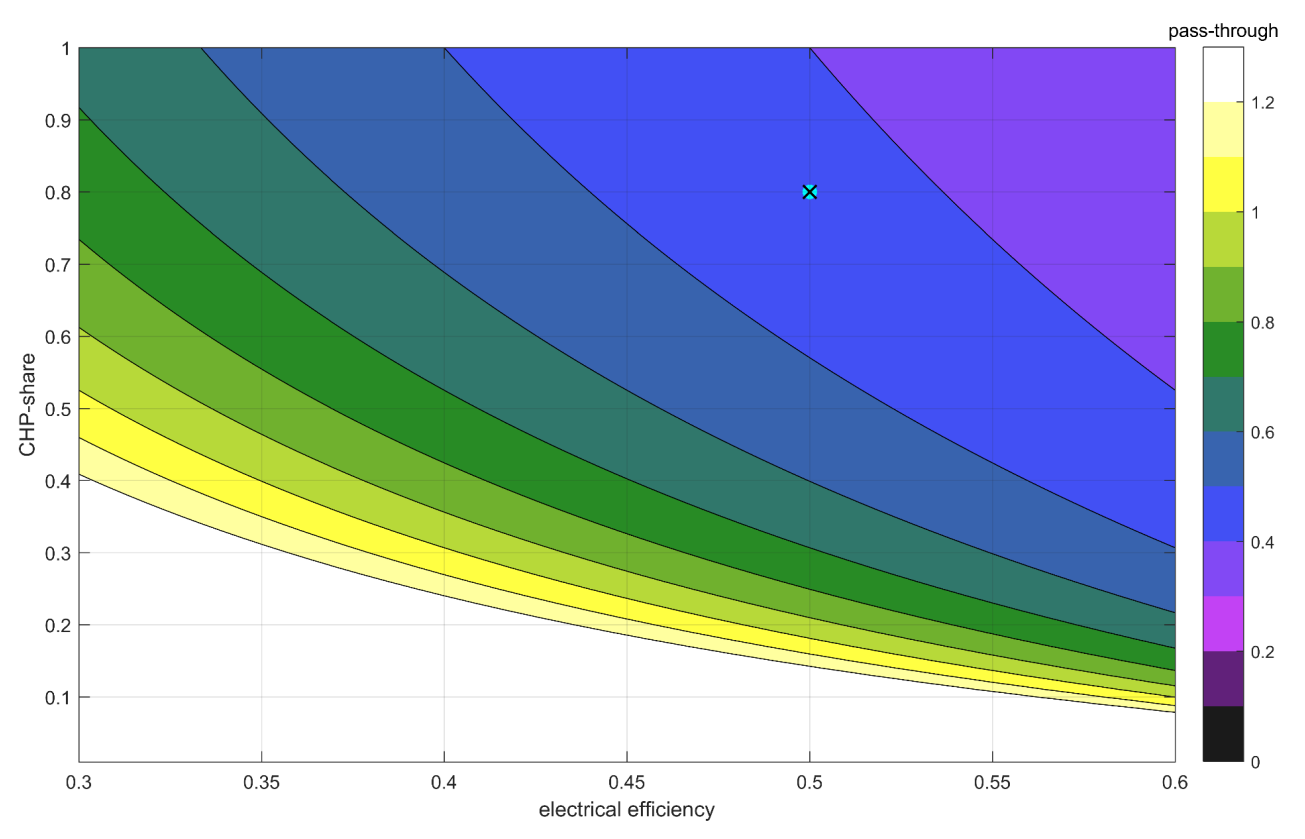
\includegraphics[scale=0.35]{Figure1_dhpt.png}
\caption{Minimally required pass-through for total cost reduction. Dot indicates the lowest pass-through level compatible with cost reduction for a district heating system with electrical efficiency of $0.5$ and a CHP heat generation share of $0.8$.}\label{Fig1}
\end{figure}

Part $\text{A}$ of the right-hand side of (\ref{8}) is strictly positive for district heating portfolios, while the sign of $\text{B}$ depends on the difference in heat cost between boilers and CHP units.
$\text{B}$ will be zero either if CHP units are capacity constrained (i.e. $\varepsilon_{s^{K}}^{p_{el}} = 0$) or if the heat cost of boilers and CHP units is equal.
If (i) CHP units have a cost advantage (cf. equation (\ref{5})) the whole of $\text{B}$ will be positive, resulting in a lower threshold for the minimally required pass-through from \ce{CO2} emission cost to electricity prices.
On the other hand, if (ii) electricity prices are so low that boilers have a cost advantage, heat will be preferentially generated in boilers, up to the available boiler capacity and heat generation from CHP units is at the minimal level.
In consequence, heat generation does not change with the electricity price, i.e. $\varepsilon_{s^K}^{p_{el}} = 0$.
This holds true until the electricity price reaches a level at which $c_{th}^{B} = c_{th}^{K}$ and we are back in case~(i).
Hence, we can restrict further analysis to the most adverse case (highest level of pass-through required for total cost reduction) in which B equals zero and (\ref{8}) simplifies to
\begin{align}\label{9}
\frac{\partial p_{el}}{\partial p_{e}} > \left( \frac{q^{T} - q^{K}}{q^{K}} \frac{\eta_{th}^{K}}{\eta_{th}^{B} \eta_{el}^{K}} + \frac{\eta_{th}^{B}}{\eta_{th}^{B} \eta_{el}^{K}} \right) em_{f}
\end{align}

Figure~\ref{Fig1} depicts the minimal total cost reducing pass-through for given shares of CHP heat generation in total emission intense heat generation and for given electrical efficiency of CHP units. 
As is to be expected, a high CHP share and high electrical efficiency both lead to lower required pass-through levels. 

As the required pass-through depends on technical characteristics of district heating systems, Table~\ref{Tab1} presents exemplary requirements on the minimal pass-through that guarantees total cost reduction.
In addition, Table~\ref{Tab1} also indicates the minimal electricity mark-up over fuel and emission cost that allows CHP plants to enjoy a cost advantage over heat boilers.
For district heating systems with the least efficient power generators, the minimal pass-through compatible with reduction of total cost is more than twice as high ($0.759$) as for district heating systems with the most efficient power generators ($0.352$).
More typical district heating systems (electrical efficiency $0.4$) are able to reduce their cost with rising emission prices, provided that at least 55.6\% of the increase in \ce{CO2} emission prices is passed on to electricity prices.

In the following, we use the power system model \emph{MEDEA} to investigate the effect of emission prices on electricity prices, i.e. to estimate the pass-through $\partial p_{el} / \partial p_{e}$. A detailed description of the model is provided in \ref{Apndx2}.
%Power plant dispatch and corresponding power prices are derived for \ce{CO2} prices of $5.89$ \euro{}/t\ce{CO2} (which is equal to the average EUA price in 2017) and all $5$ \euro{}/t\ce{CO2} increments up to $80.89$ \euro{}/t\ce{CO2}, given the current inventory of power plants.
%The results are used to approximate $\partial p_{el} / \partial p_{e} \approxeq \Delta p_{el} / \Delta p_{e}$, the pass-through from emission prices to electricity prices.

\begin{table}[t]
\caption{Effects of technical parameters on heat generation units}
\smallskip
\centering
\begin{tabular}{c c c}
\hline
\makecell{Electrical \\efficiency} & \makecell{Min. mark-up \\(cf. eq. (\ref{5}))} &
\makecell{Min. pass-through \\ (cf. eq. (\ref{9}))} \\ [1.5 ex]
\hline  \hline
$0.3$ & $0.481$ & $0.759$ \\ [0.5 ex] \hline
$0.4$ & $0.389$ & $0.556$ \\ [0.5 ex] \hline
$0.5$ & $0.333$ & $0.433$ \\ [0.5 ex] \hline
$0.6$ & $0.296$ & $0.352$ \\ [1.0 ex]
\hline \hline
\end{tabular}
\label{Tab1}
\end{table}

\section{Results} \label{sec_results}
To approximate pass-through rates from \ce{CO2} emission costs to electricity prices, we determine dispatch of installed power plant capacities in $16$ emission price scenarios $s = 0,1,\ldots,15$, both for the current and a projected future electricity system.
In either setting, we start from actually observed daily EU emission allowance prices (annual average in 2017: $5.89$ \euro{}/t\ce{CO2}) and increase the price by $5$ \euro{}/t\ce{CO2} in each subsequent scenario up to an annual average price of $80.89$ \euro{}/t\ce{CO2}, leaving everything else unchanged.
The marginals on the electricity supply and demand balance equation (see equation (\ref{12}) in~\ref{Apndx2}) of our power system model reflect the endogenously determined hourly electricity prices.
We use the electricity base price $p_{el}$ (i.e. the annual average of the hourly spot price) to approximate the pass-through from emission costs to electricity prices by
\begin{align}\label{10}
\frac{\Delta p_{el}}{\Delta p_{e}} = \frac{p_{el, s} - p_{el, s-1}}{p_{e, s} - p_{e, s-1}}
\end{align} 


\subsection{Effects of increasing emission prices in the current electricity system}
Our pass-through estimates for the electricity system as of 2017 are presented in Figure \ref{Fig3}, once for the current system allowing for power generation from all installed capacities and once for the current system with restricted operable capacities, e.g. due to maintenance. 
The possibility to substitute electricity generation from emission intense generators with electricity generation from low-emitting units affects pass-through estimates considerably.
If substitution is impossible, emission cost pass-through will be constant. 
With limited potential for substitution, cost pass-through can increase as emission prices rise. This happens when emission intense generators, e.g. lignite-fired plants, are inframarginal at low emission prices. As emission prices increase, marginal cost of these units rise strongly. At some emission price, one of these units will be the price setting, most expensive still dispatched unit. As emission prices increase further, this unit would be priced out of the market if sufficient capacity for replacing this unit would be available. 
However, in the absence of substitution potential, emission cost pass-through will remain high.

In the following, we will confine our attention to the more interesting case in which generation capacities can be substituted up to installed capacities. 
In this case, emission cost pass-through to electricity prices depends on the absolute level of the emission price, and is declining from $0.82$ at emission prices between $5$ and $10$ \euro{}/t\ce{CO2} to $0.64$ at emission prices between $50$ and $55$~\euro{}/t\ce{CO2}.

\begin{figure}[t]
\centering
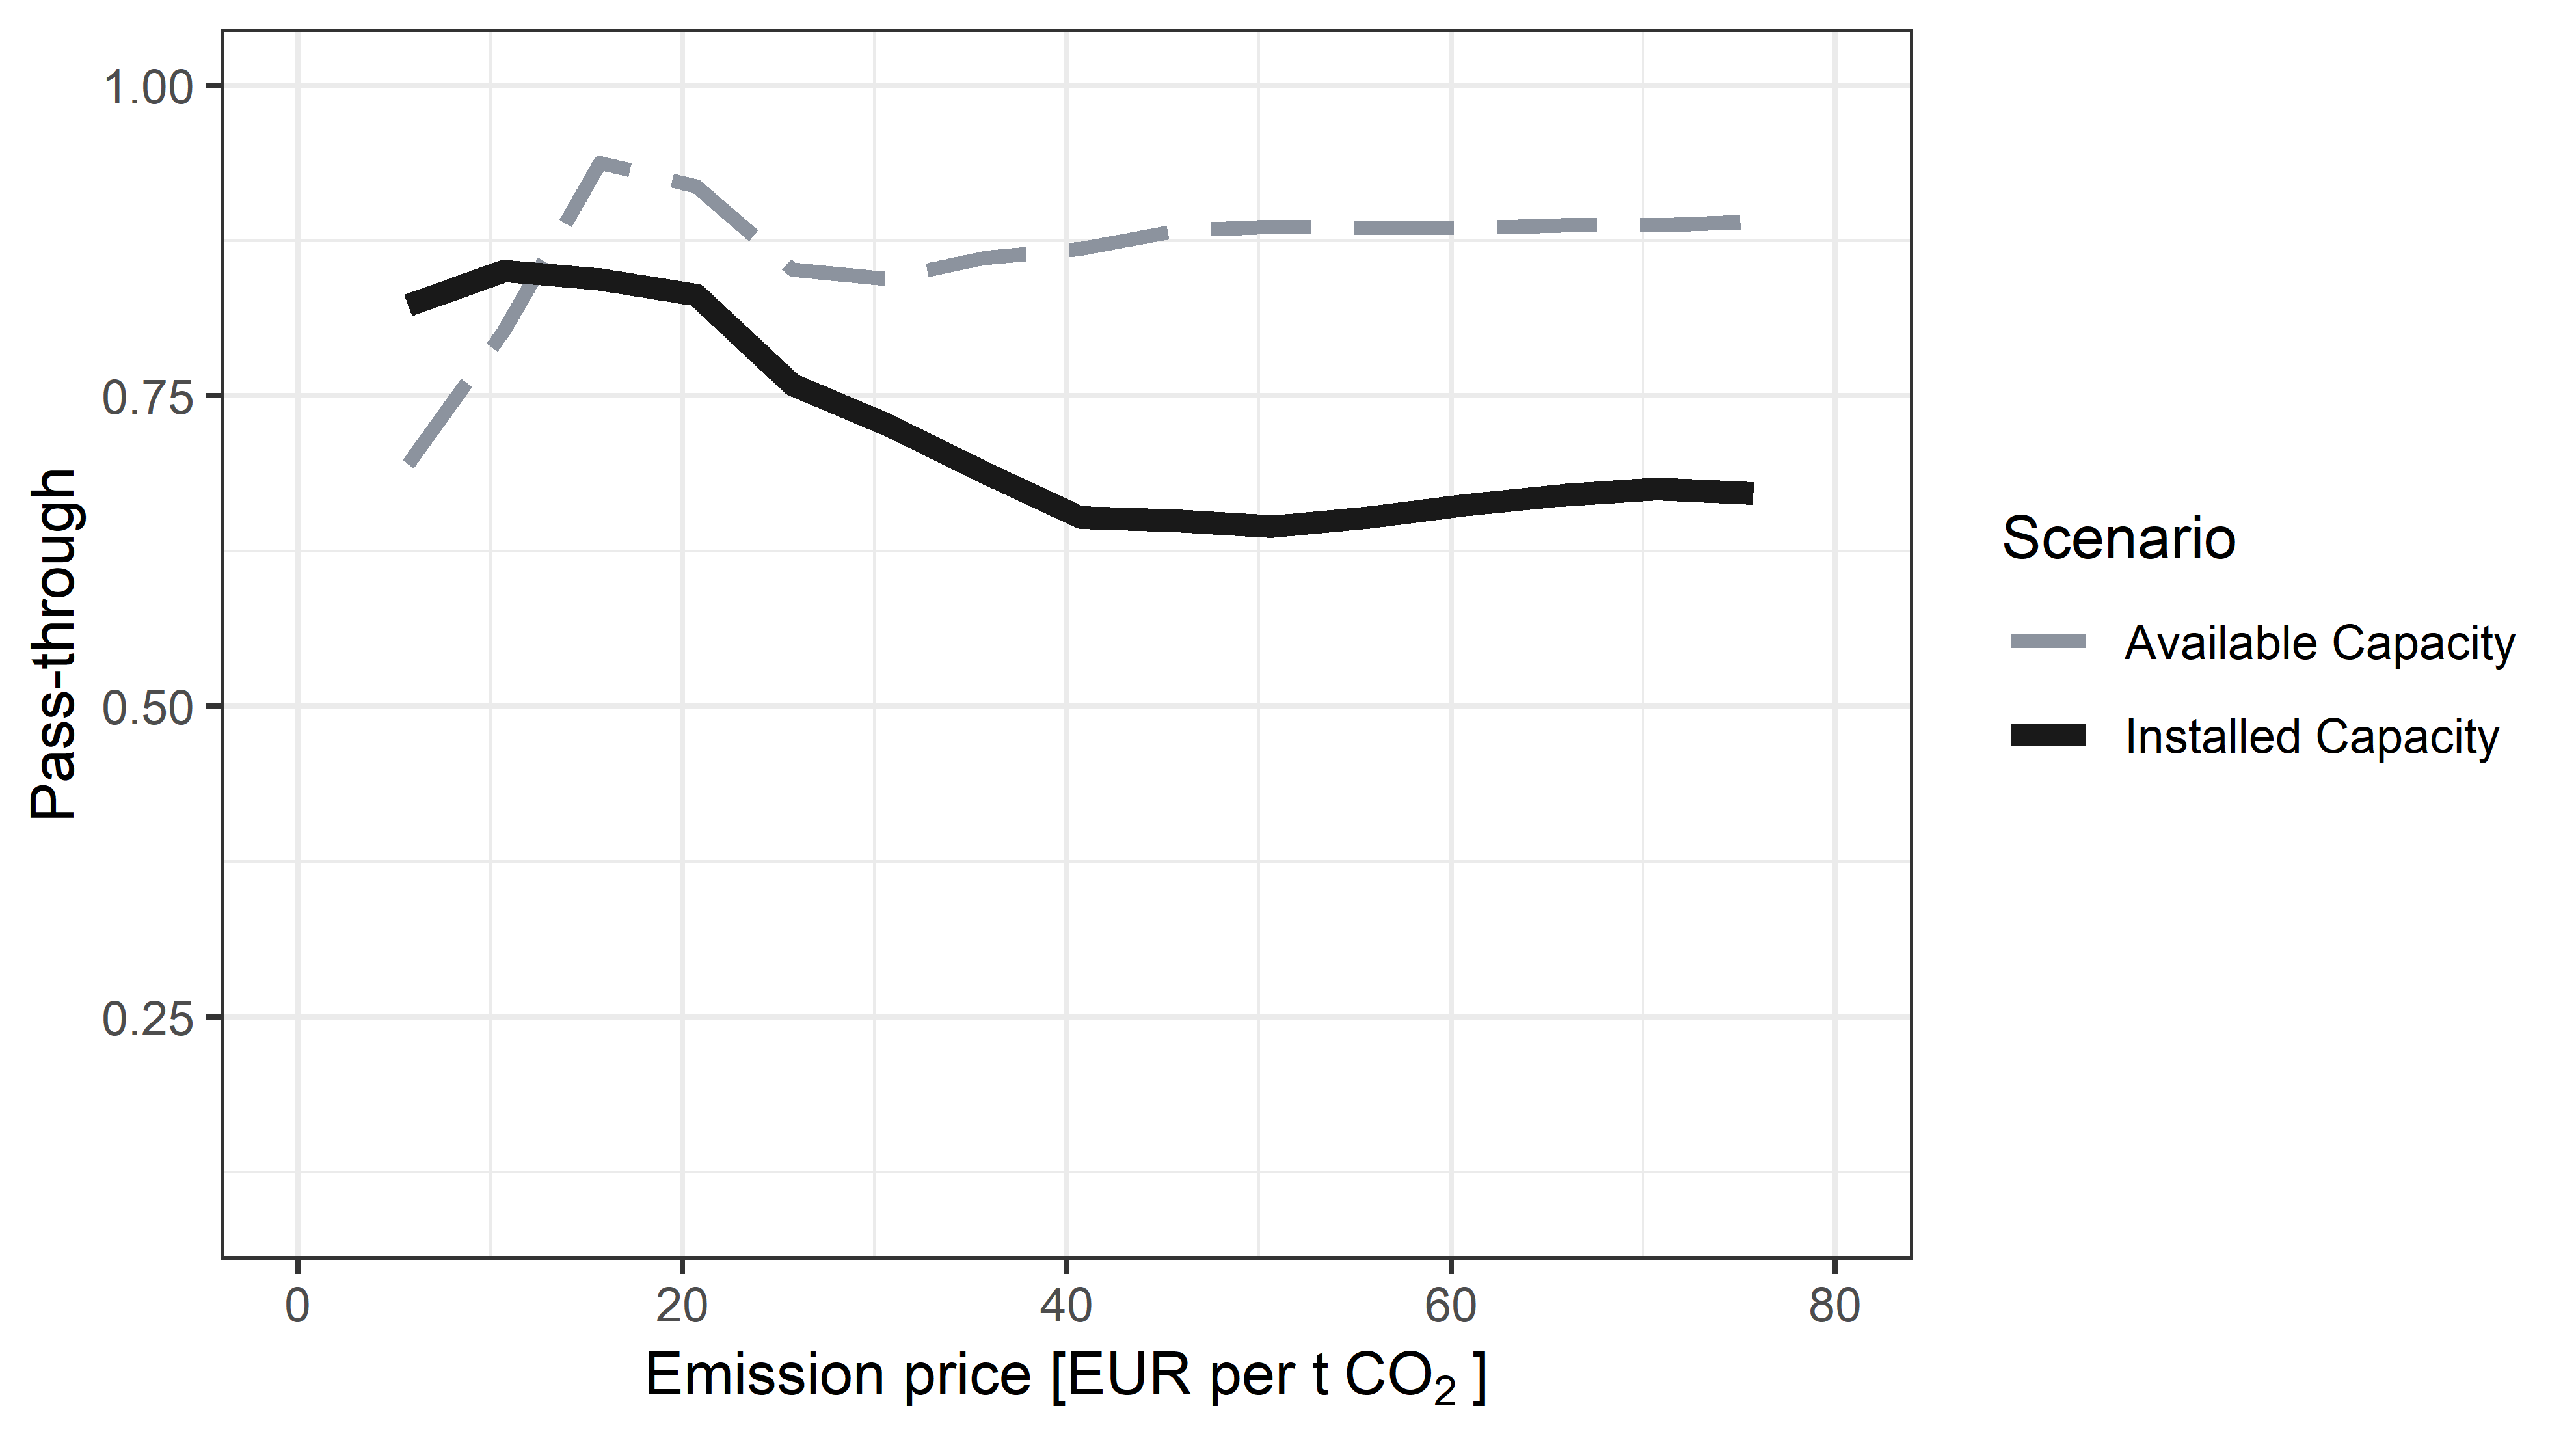
\includegraphics[scale=0.75]{Figure3a_current_capacity.png}
\caption{Estimated pass-through from emission prices to electricity prices (2017)}\label{Fig3}
\end{figure}

The co-movement of \ce{CO2} emission prices and the pass-through can be explained by (i) a 'fuel switch' triggered by rising emissions prices, (ii) a 'CHP generation switch' and (iii) an increase in the overall fuel efficiency.

The 'fuel switch' (i) in response to increasing emission costs is illustrated in Figure~\ref{Fig4a}.
At low \ce{CO2} prices, lignite and coal fired power plants dominate the generation mix, with approximately $440$ TWh of lignite and $277$ TWh of hard coal  being burned over the course of the year.
Price-setting marginal power plants are predominantly fueled by coal and natural gas.
With emission prices rising above $20$~\euro{}/t\ce{CO2}, generation cost of lignite-fired plants increase disproportionately strong, as lignite is the fuel with the highest specific \ce{CO2} emissions. 
In effect, lignite-fired generation becomes more expensive relative to generation from coal and natural gas.
While some lignite-fired units are driven out of the market, the remaining units are increasingly often becoming the price setting, marginal (i.e. most expensive still dispatched) units.

\begin{figure}[t]
\centering
\begin{subfigure}[t]{0.475\textwidth}
\centering
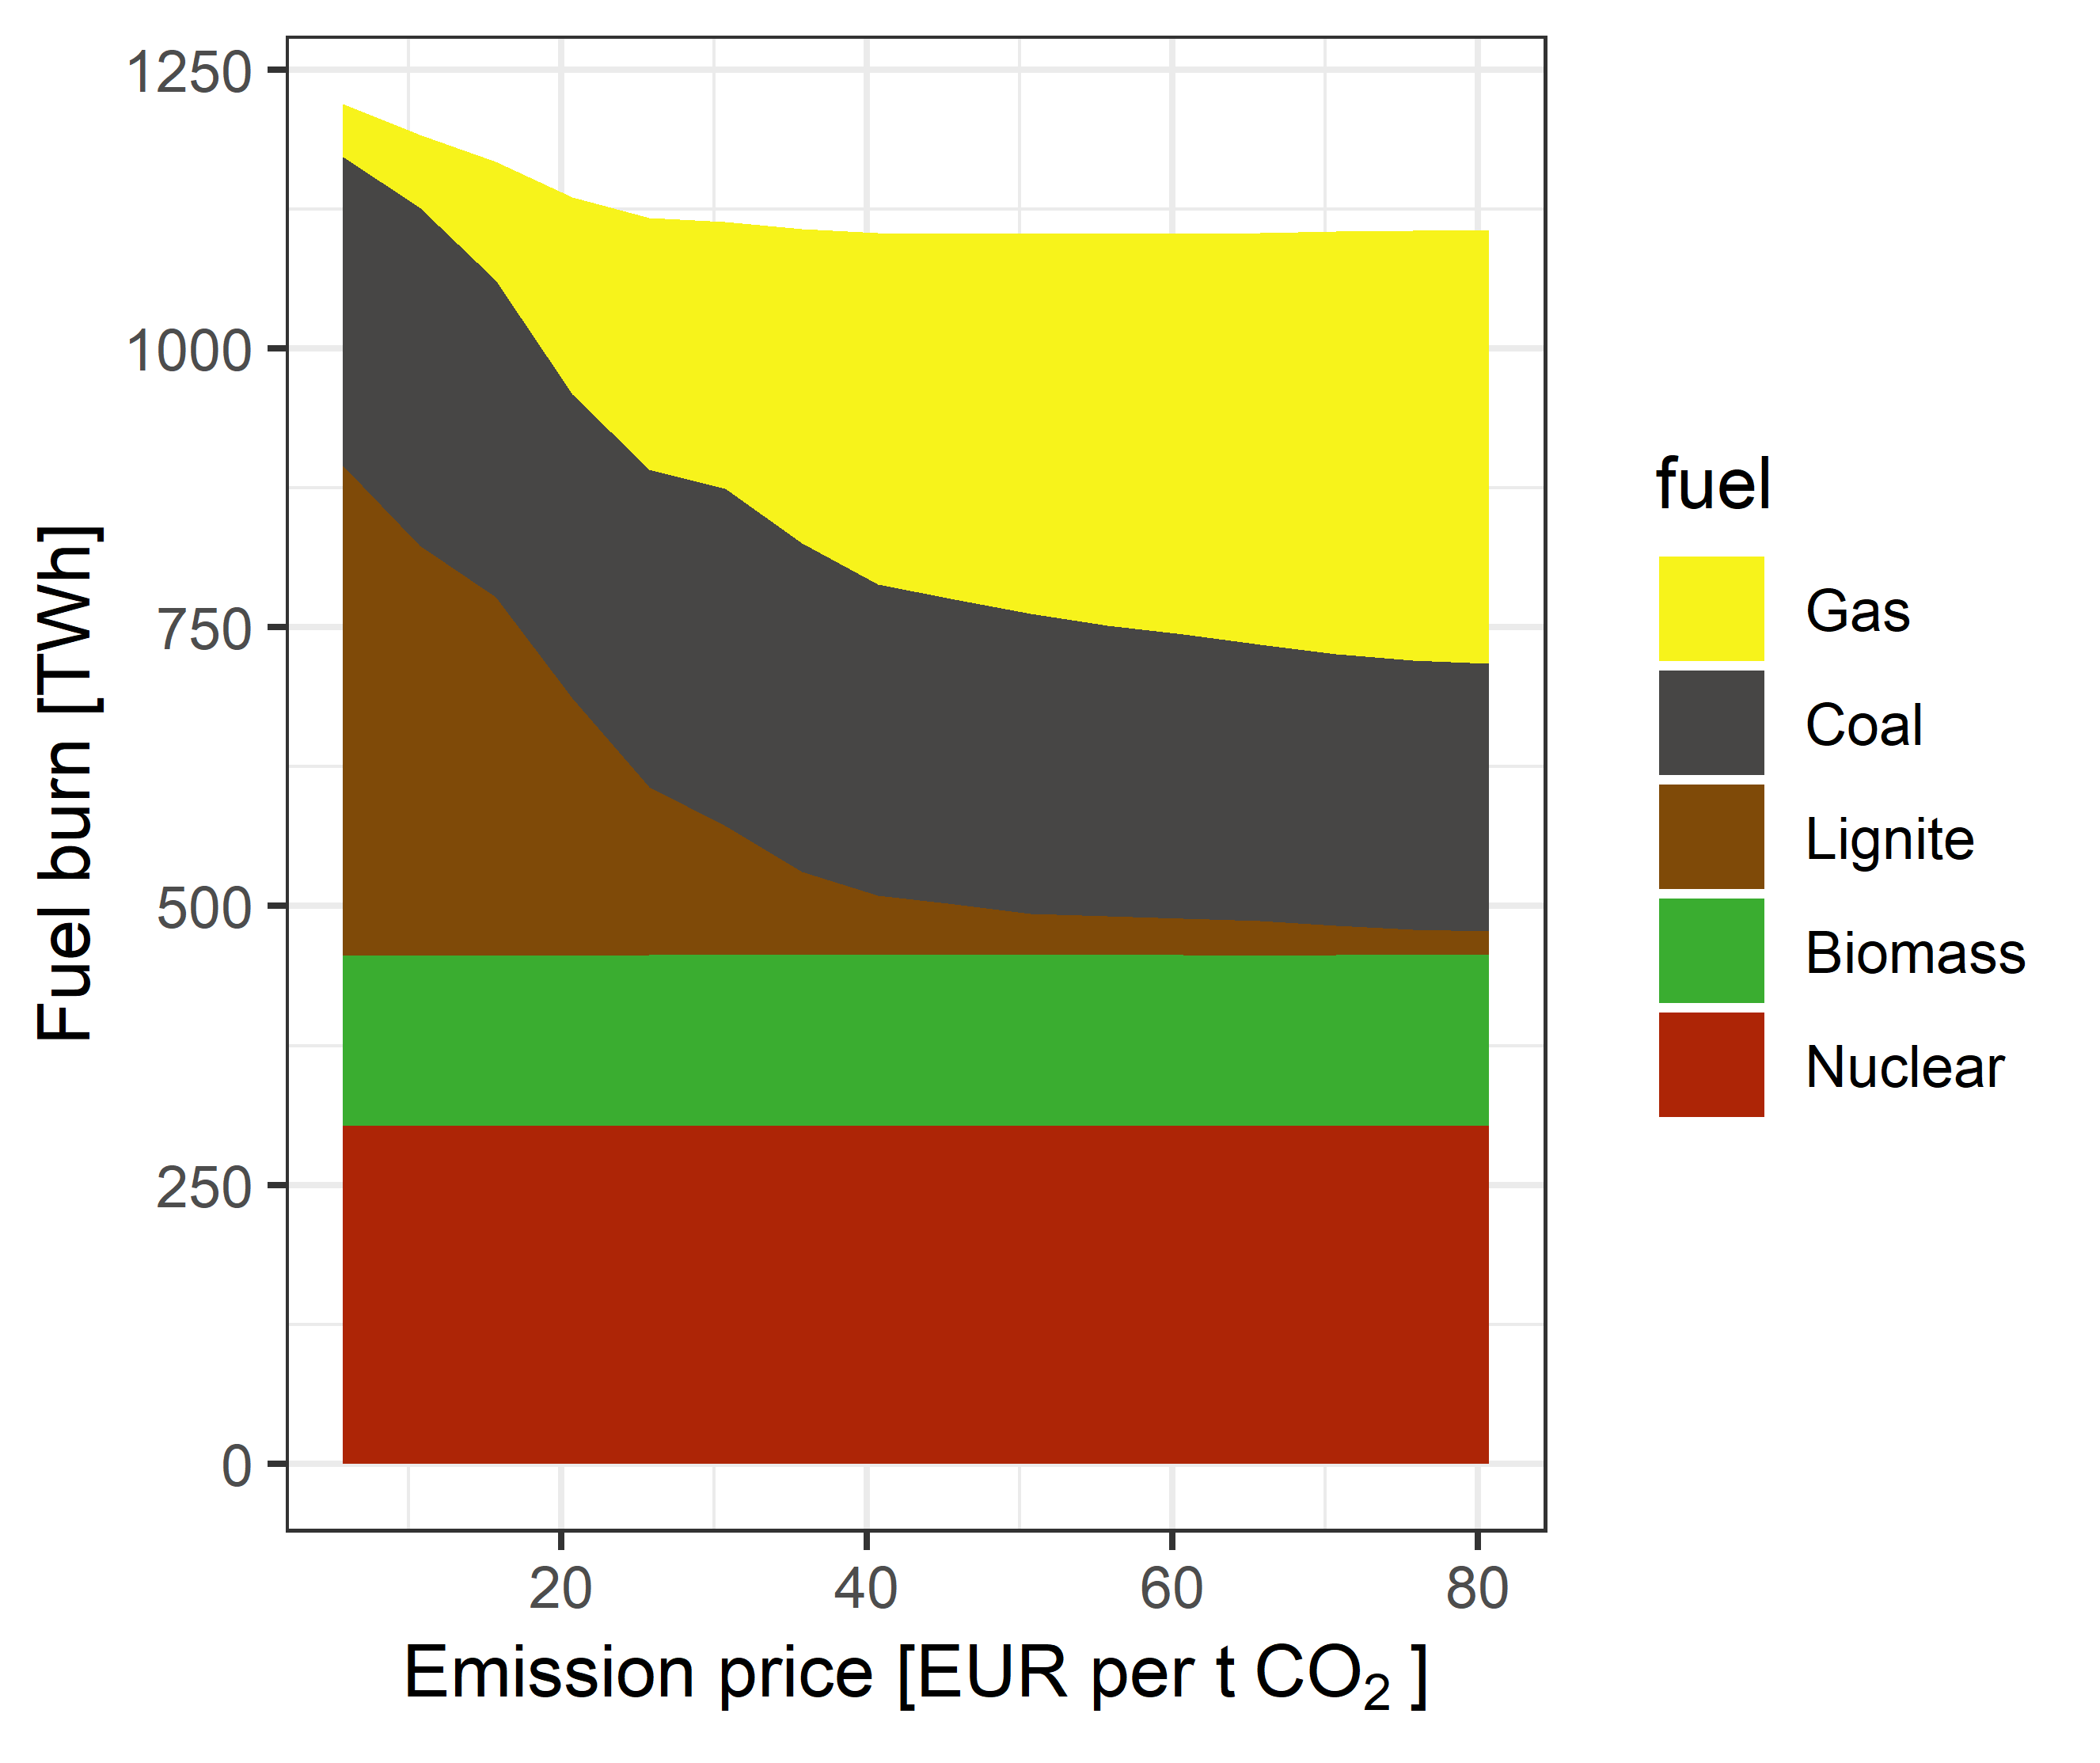
\includegraphics[scale=0.75]{Figure4a_fuel_burn.png}
\caption{Fuel burn for power generation} \label{Fig4a}
\end{subfigure}
%~
\begin{subfigure}[t]{0.475\textwidth}
\centering
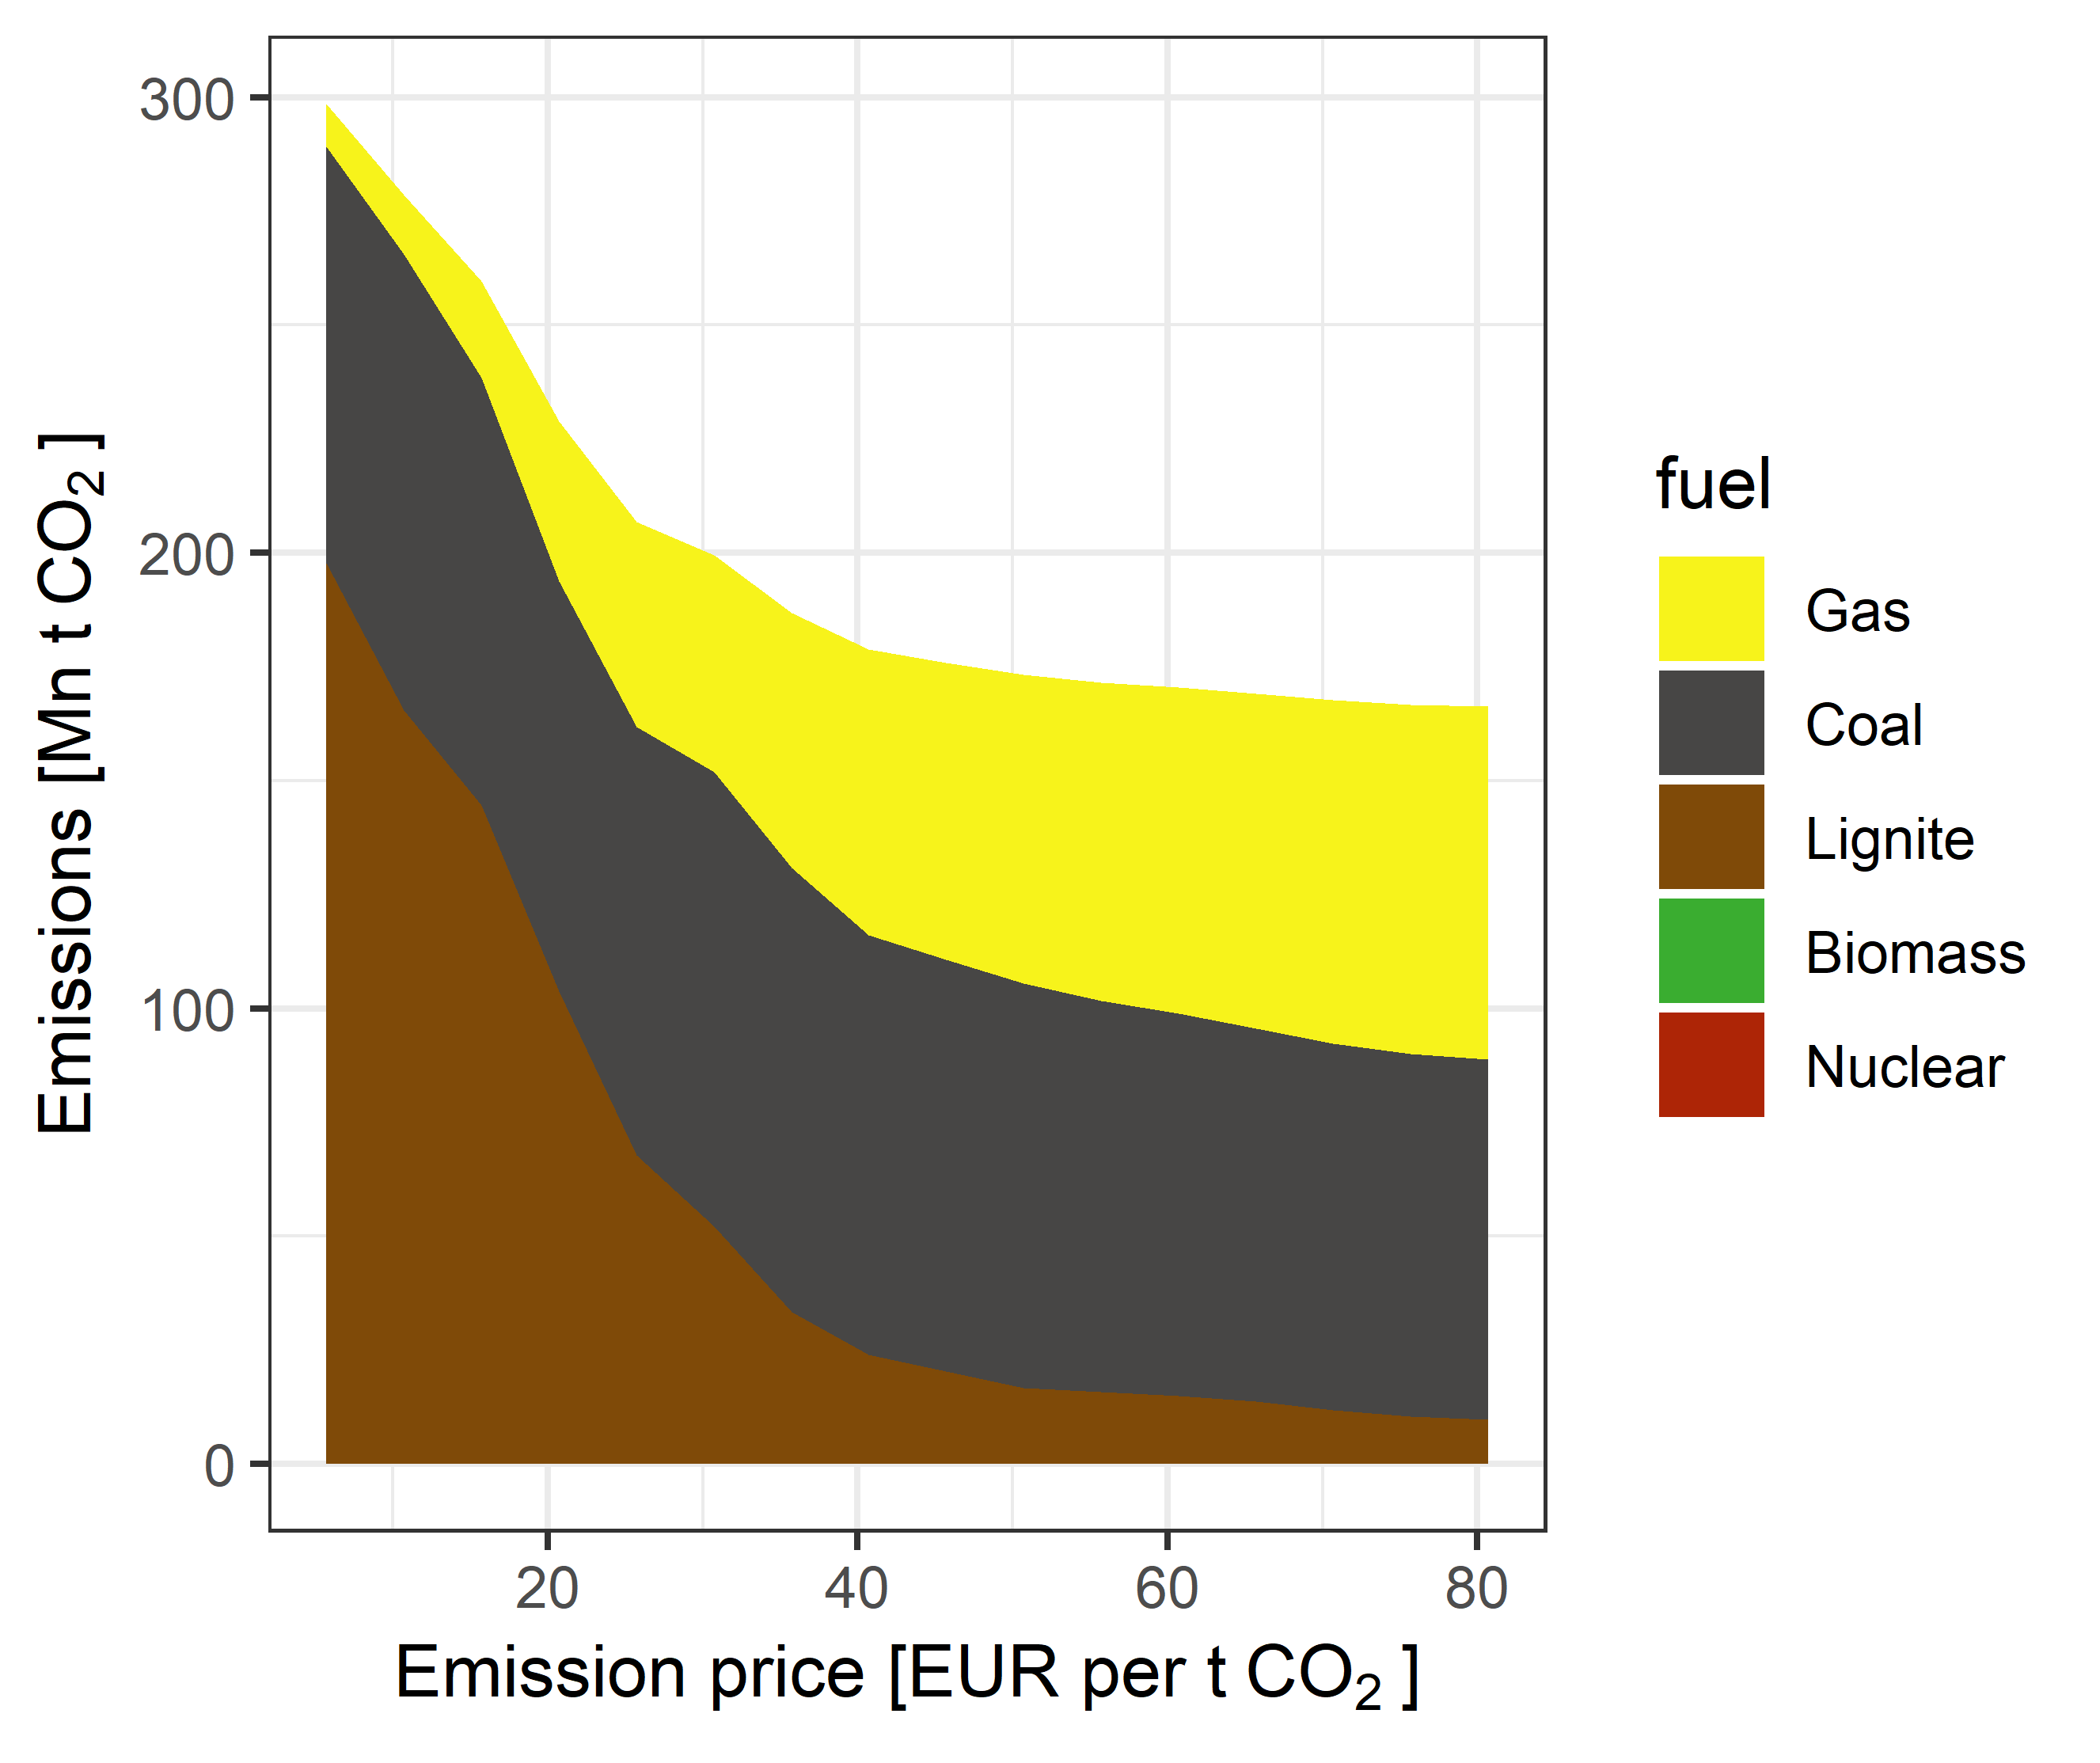
\includegraphics[scale=0.75]{Figure4b_emissions.png}
\caption{\ce{CO2} emissions from power generation}\label{Fig4b}
\end{subfigure}
\caption{Results from emission price scenarios}\label{Fig4}
\end{figure}

At emission prices at or above $20$~\euro{}/t\ce{CO2}, lignite loses most of its cost advantage relative to coal and natural gas and the use of lignite for power generation begins to decline markedly.
Under these conditions, lignite-fired units are frequently the most expensive dispatched units.
In consequence, any further increase in \ce{CO2} emission prices leads to a particularly strong effect on electricity prices.
However, this effect vanishes as more and more lignite-fired generators become uncompetitive and cease generation.
With \ce{CO2} emission prices reaching $40$~\euro{}/t\ce{CO2}, the decline in lignite use slows down.
Further emission reductions are caused by the substitution of lignite and coal fired plants with natural gas fired generators.
However, even for emission prices above $70$~\euro{}/t\ce{CO2} coal and lignite account for roughly one quarter of total thermal power generation as the power plant stock is fixed in our analysis and cannot adjust to higher \ce{CO2} emission costs.

The 'CHP generation switch' (ii) occurs in parallel to the fuel switch.
In response to rising emission prices, the cost of power generation from emission intense lignite increases particularly, leading to a marked decline of power generation (but a slight increase in heat generation) from these units. This is compensated by additional power generation from natural gas and hard coal. While natural gas-fired units expand their fuel use to raise their output of electricity and heat, hard coal-fired co-generation units shift their output from heat towards power. 
In total, less lignite is burned ($-27\%$as emission prices rise from $5.89$~\euro{}/t\ce{CO2} to $15.89$~\euro{}/t\ce{CO2}), but with higher total efficiency (total generation declines only by $-15\%$ over the same price range). 
Conversely, burning of hard coal and natural gas increases by $2.6$\% and $124.6$\%, respectively.

In addition, we observe (iii) an increase in overall fuel efficiency, as visible in Figure~\ref{Fig4a}.
Total fuel combustion for power generation declines from $1219$ TWh at low emission prices to $1106$ TWh at the highest \ce{CO2} emission prices that we investigated.
Taken together, these effects induce relatively steep marginal \ce{CO2} emission reductions for emission prices up to $20$~\euro{}/t\ce{CO2} (see Figure~\ref{Fig4b}).
Above this price level marginal \ce{CO2} emission reductions gradually level off as the substitution potential for lignite-fired generators vanishes. 
At emission prices above $40$~\euro{}/t\ce{CO2} most of the (short-run) substitution potential is exploited and marginal \ce{CO2}~emission reductions recede considerably.

\subsection{Robustness of estimates}\label{robustn}
To assess the robustness of our pass-through estimates with respect to model assumptions, we conduct sensitivity runs, in which we vary the parameter(s) of interest, holding everything else constant.
Figure~\ref{Fig5} summarizes all resulting estimates for the pass-through from \ce{CO2} emission costs to electricity prices.
\begin{figure}[t]
\centering
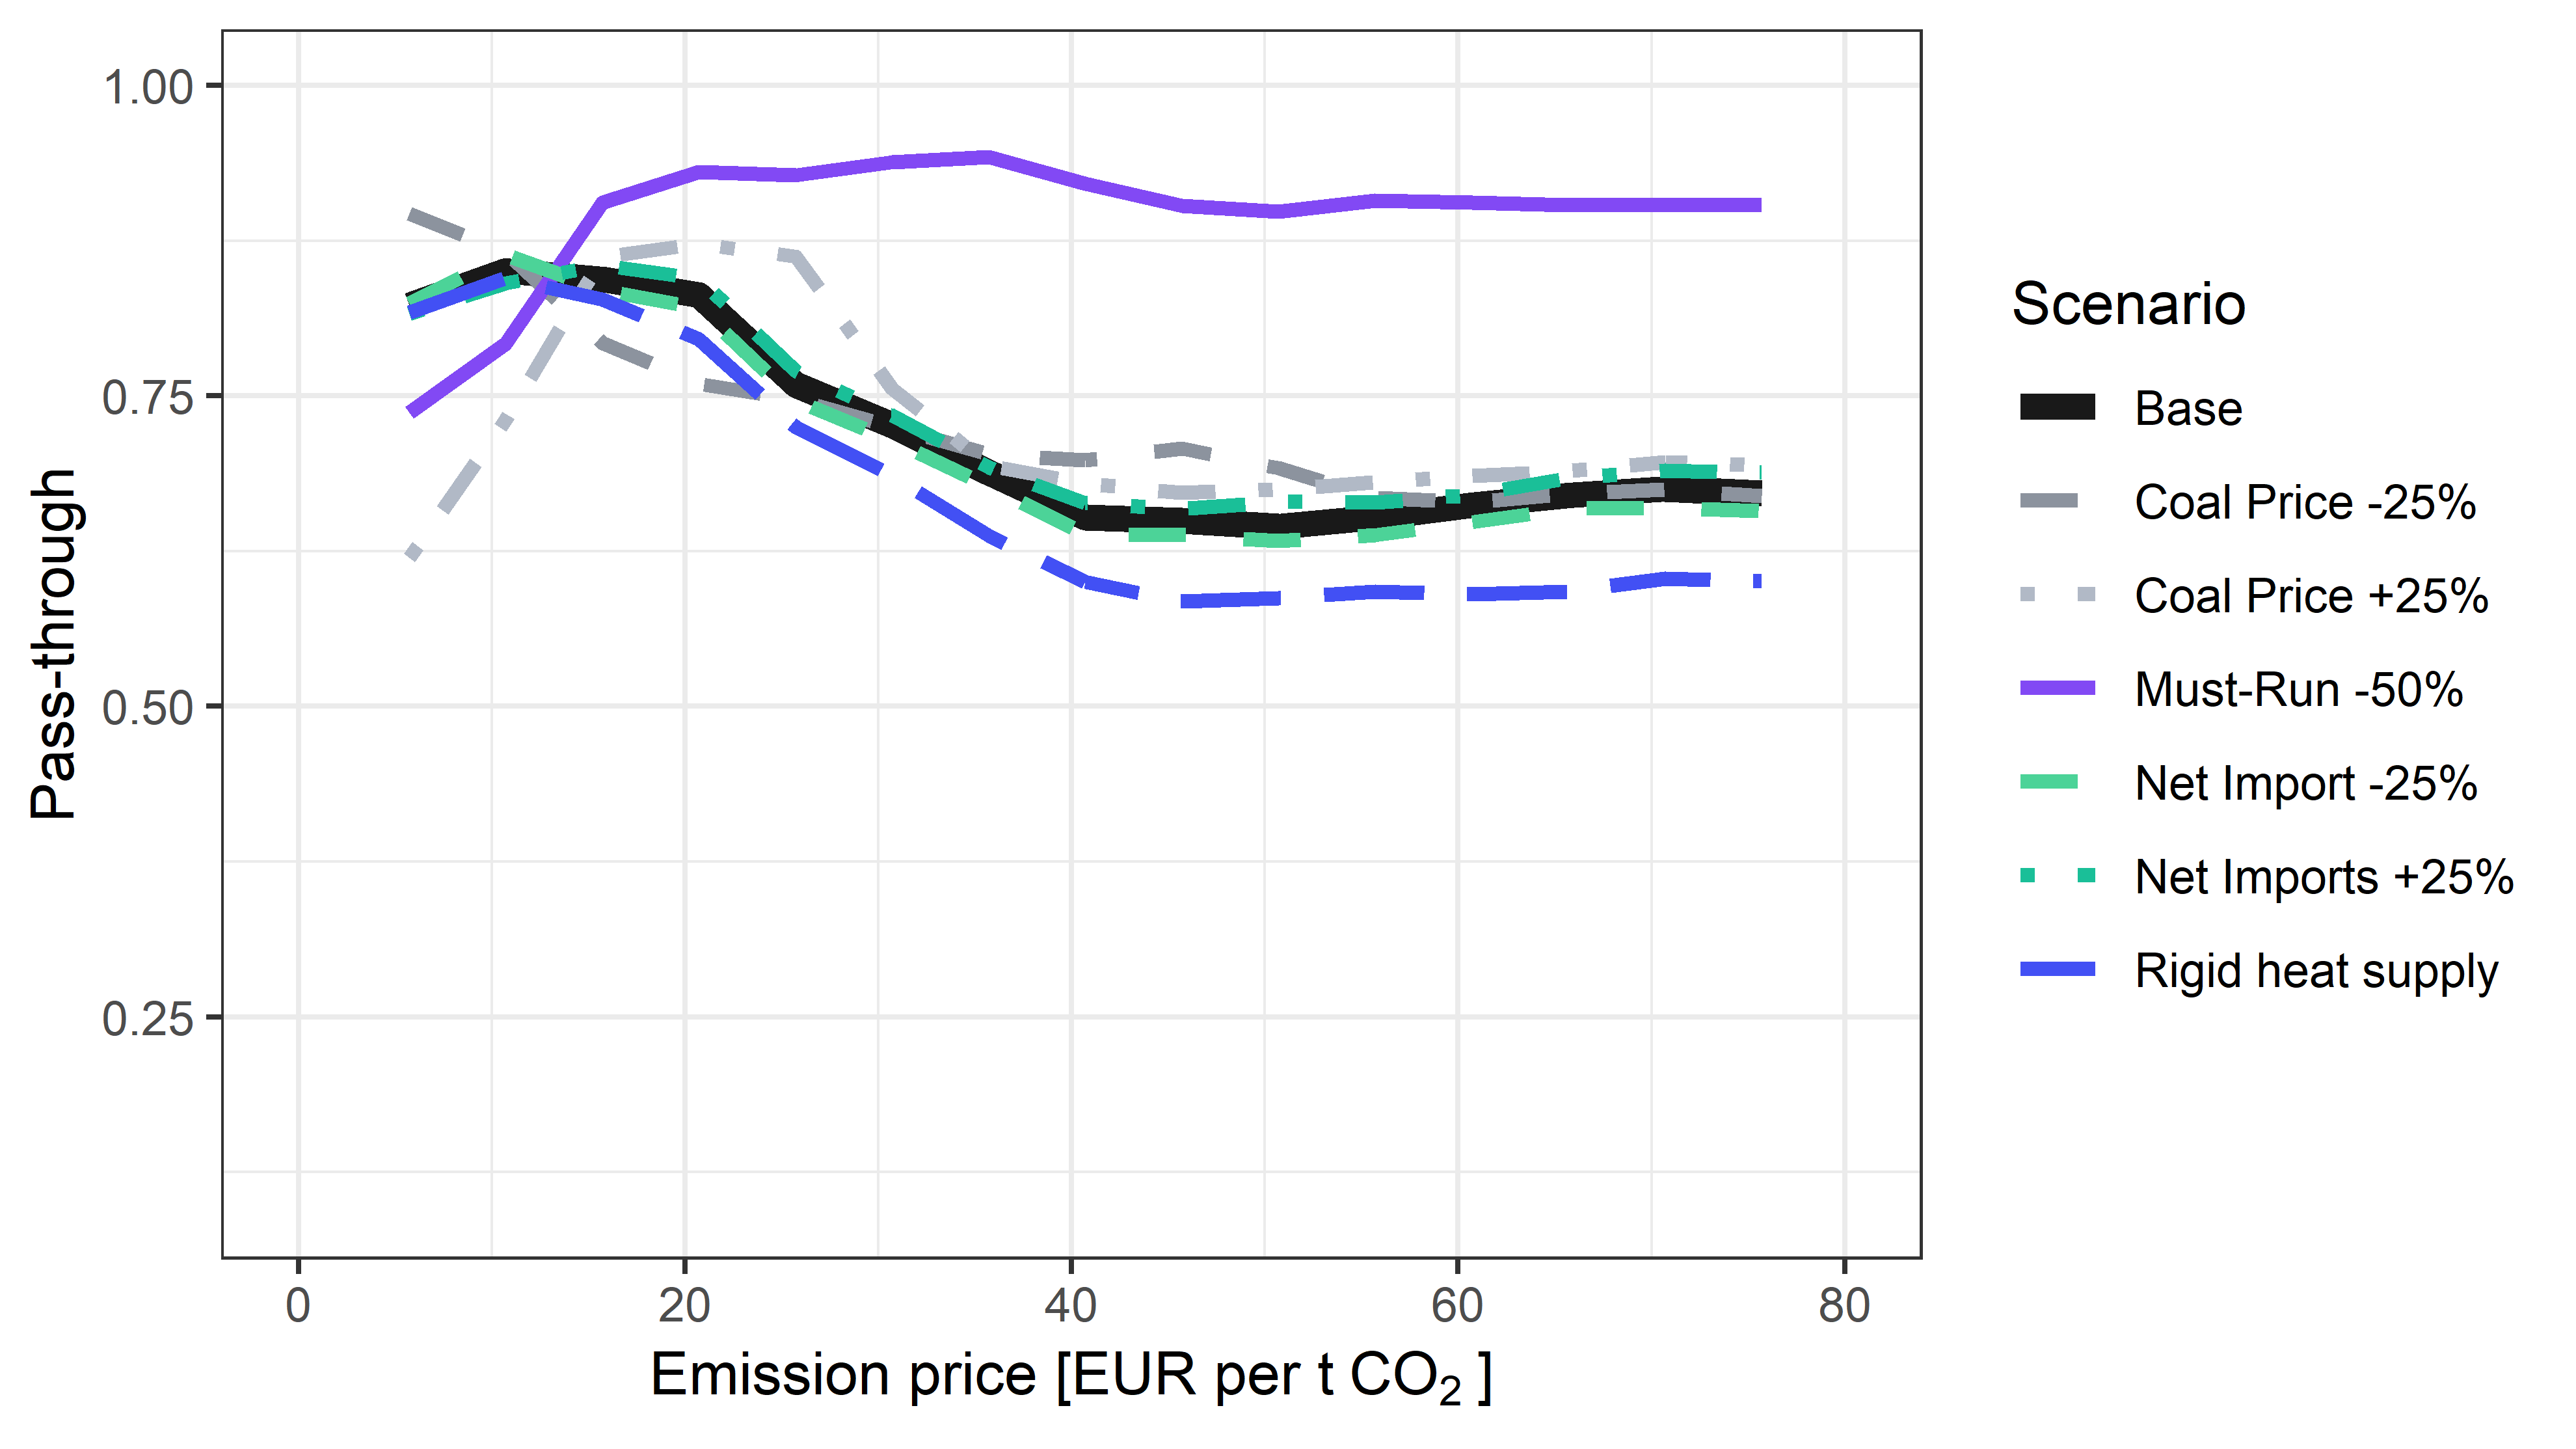
\includegraphics[scale=0.75]{Figure3c_current_sensitivity.png}
\caption{Sensitivity of pass-through estimates}\label{Fig5}
\end{figure}
\subsubsection*{International electricity exchange}
  
An increase of $25\%$ in net imports (quantities imported less quantities exported) leads to an average increase in the emission cost pass-through by $0.01$ compared to our baseline estimate.
Germany was a net exporter of electricity in 2017, i.e. over the course of the year electricity generation was higher than it would have been in the absence of international electricity exchange. 
Ceteris paribus, this marginal generation has to be sourced from thermal generators. In effect, the emission cost pass-through increases.

\subsubsection*{Relative price of coal}
We find that a $25\%$ increase in (relative) coal prices has a considerable impact on the emission cost pass-through at low emission prices. The higher price of coal relative to natural gas induces a $26$ TWh shift in power generation from coal to natural gas, as compared to our baseline. In effect, marginal plants are more frequently natural gas-fired, leading to initially lower pass-through levels. As the specific \ce{CO2} emissions of coal are about two-thirds higher than those of natural gas, rising emission prices lead to a disproportionate increase in the marginal cost of coal-fired generators. In effect, such generators are increasingly often the marginal (most expensive still dispatched) unit, inducing a rising pass-though level. At high emission prices, emission cost dominates fuel cost and the effect on the pass-through recedes.

\subsubsection*{Ancillary Services and system flexibility} 
Lowering the capacity required to be operational at any point in time for the provision of ancillary services by $50\%$ increases our estimated pass-through on average by $0.19$.
The minimum capacity requirement for the provision of ancillary services is effective only if the residual electricity demand falls below the minimal capacity level.
In this case, supply and demand must be balanced either through curtailment of renewable electricity generation (which would raise residual demand) or through increased pumping by pumped hydro storages (which has the additional benefit that ancillary services can also be provided through pumping).
In consequence, the marginal, price-setting unit is a renewable generator and the cost of \ce{CO2} emissions is not passed through at that time.
With less capacity required to be operational for the provision of ancillary services, such incidents occur less frequently and thermal, \ce{CO2} emission intense generators are setting the price more often. This results in a higher emission cost pass-through.\subsubsection*{Rigidity of heat supply}
To examine the effect of fully substitutability of heat generation sources, we introduce a lower bound on the hourly generation of heat from lignite and coal that is proportional to the fuels’ share in total installed CHP heat generation capacity.
For emission prices up to $15$~\euro{}/t\ce{CO2} this has little effect on our pass-through estimates, as emission intense generators are anyway dispatched. 
At higher emission prices, the constraint gets binding, requiring emission intense generators to be dispatched. In effect, less emission intense generators are determining the price and emission cost pass-through declines by up to $0.07$.

\subsection{Effect of \ce{CO2} prices in a future electricity system}
The power system undergoes rapid changes, as renewable electricity generation is added to the system while generation from fossil power plants retreats. In Germany, the Renewable Energy Act~\citep{EEG2017} governs the further expansion of renewable electricity generation. In addition, the government-installed, so-called “Coal Commission” recently proposed to limit power generation from coal and lignite and eventually end it by 2038 \citep{KommissionWSB2019}.
In line with these plans, we assume that by 2030 electricity generation from solar PV and wind turbines will increase by $70\%$ and $100\%$, respectively. Over the same time period, coal and lignite fired generation capacities are assumed to be reduced to $35\%$ and $45\%$ of capacities installed in 2017 while nuclear generation is already phased-out. 
In addition, we simulate a scenario for 2040, which assumes an end to power generation from coal and lignite, while generation from wind energy increases by more than 140\% and solar photovoltaics by 130\% as compared to our base year 2017. 
For all scenarios, we assume sufficient additional natural gas-fired generation capacities so as to guarantee resource adequacy.
\begin{figure}[t]
\centering
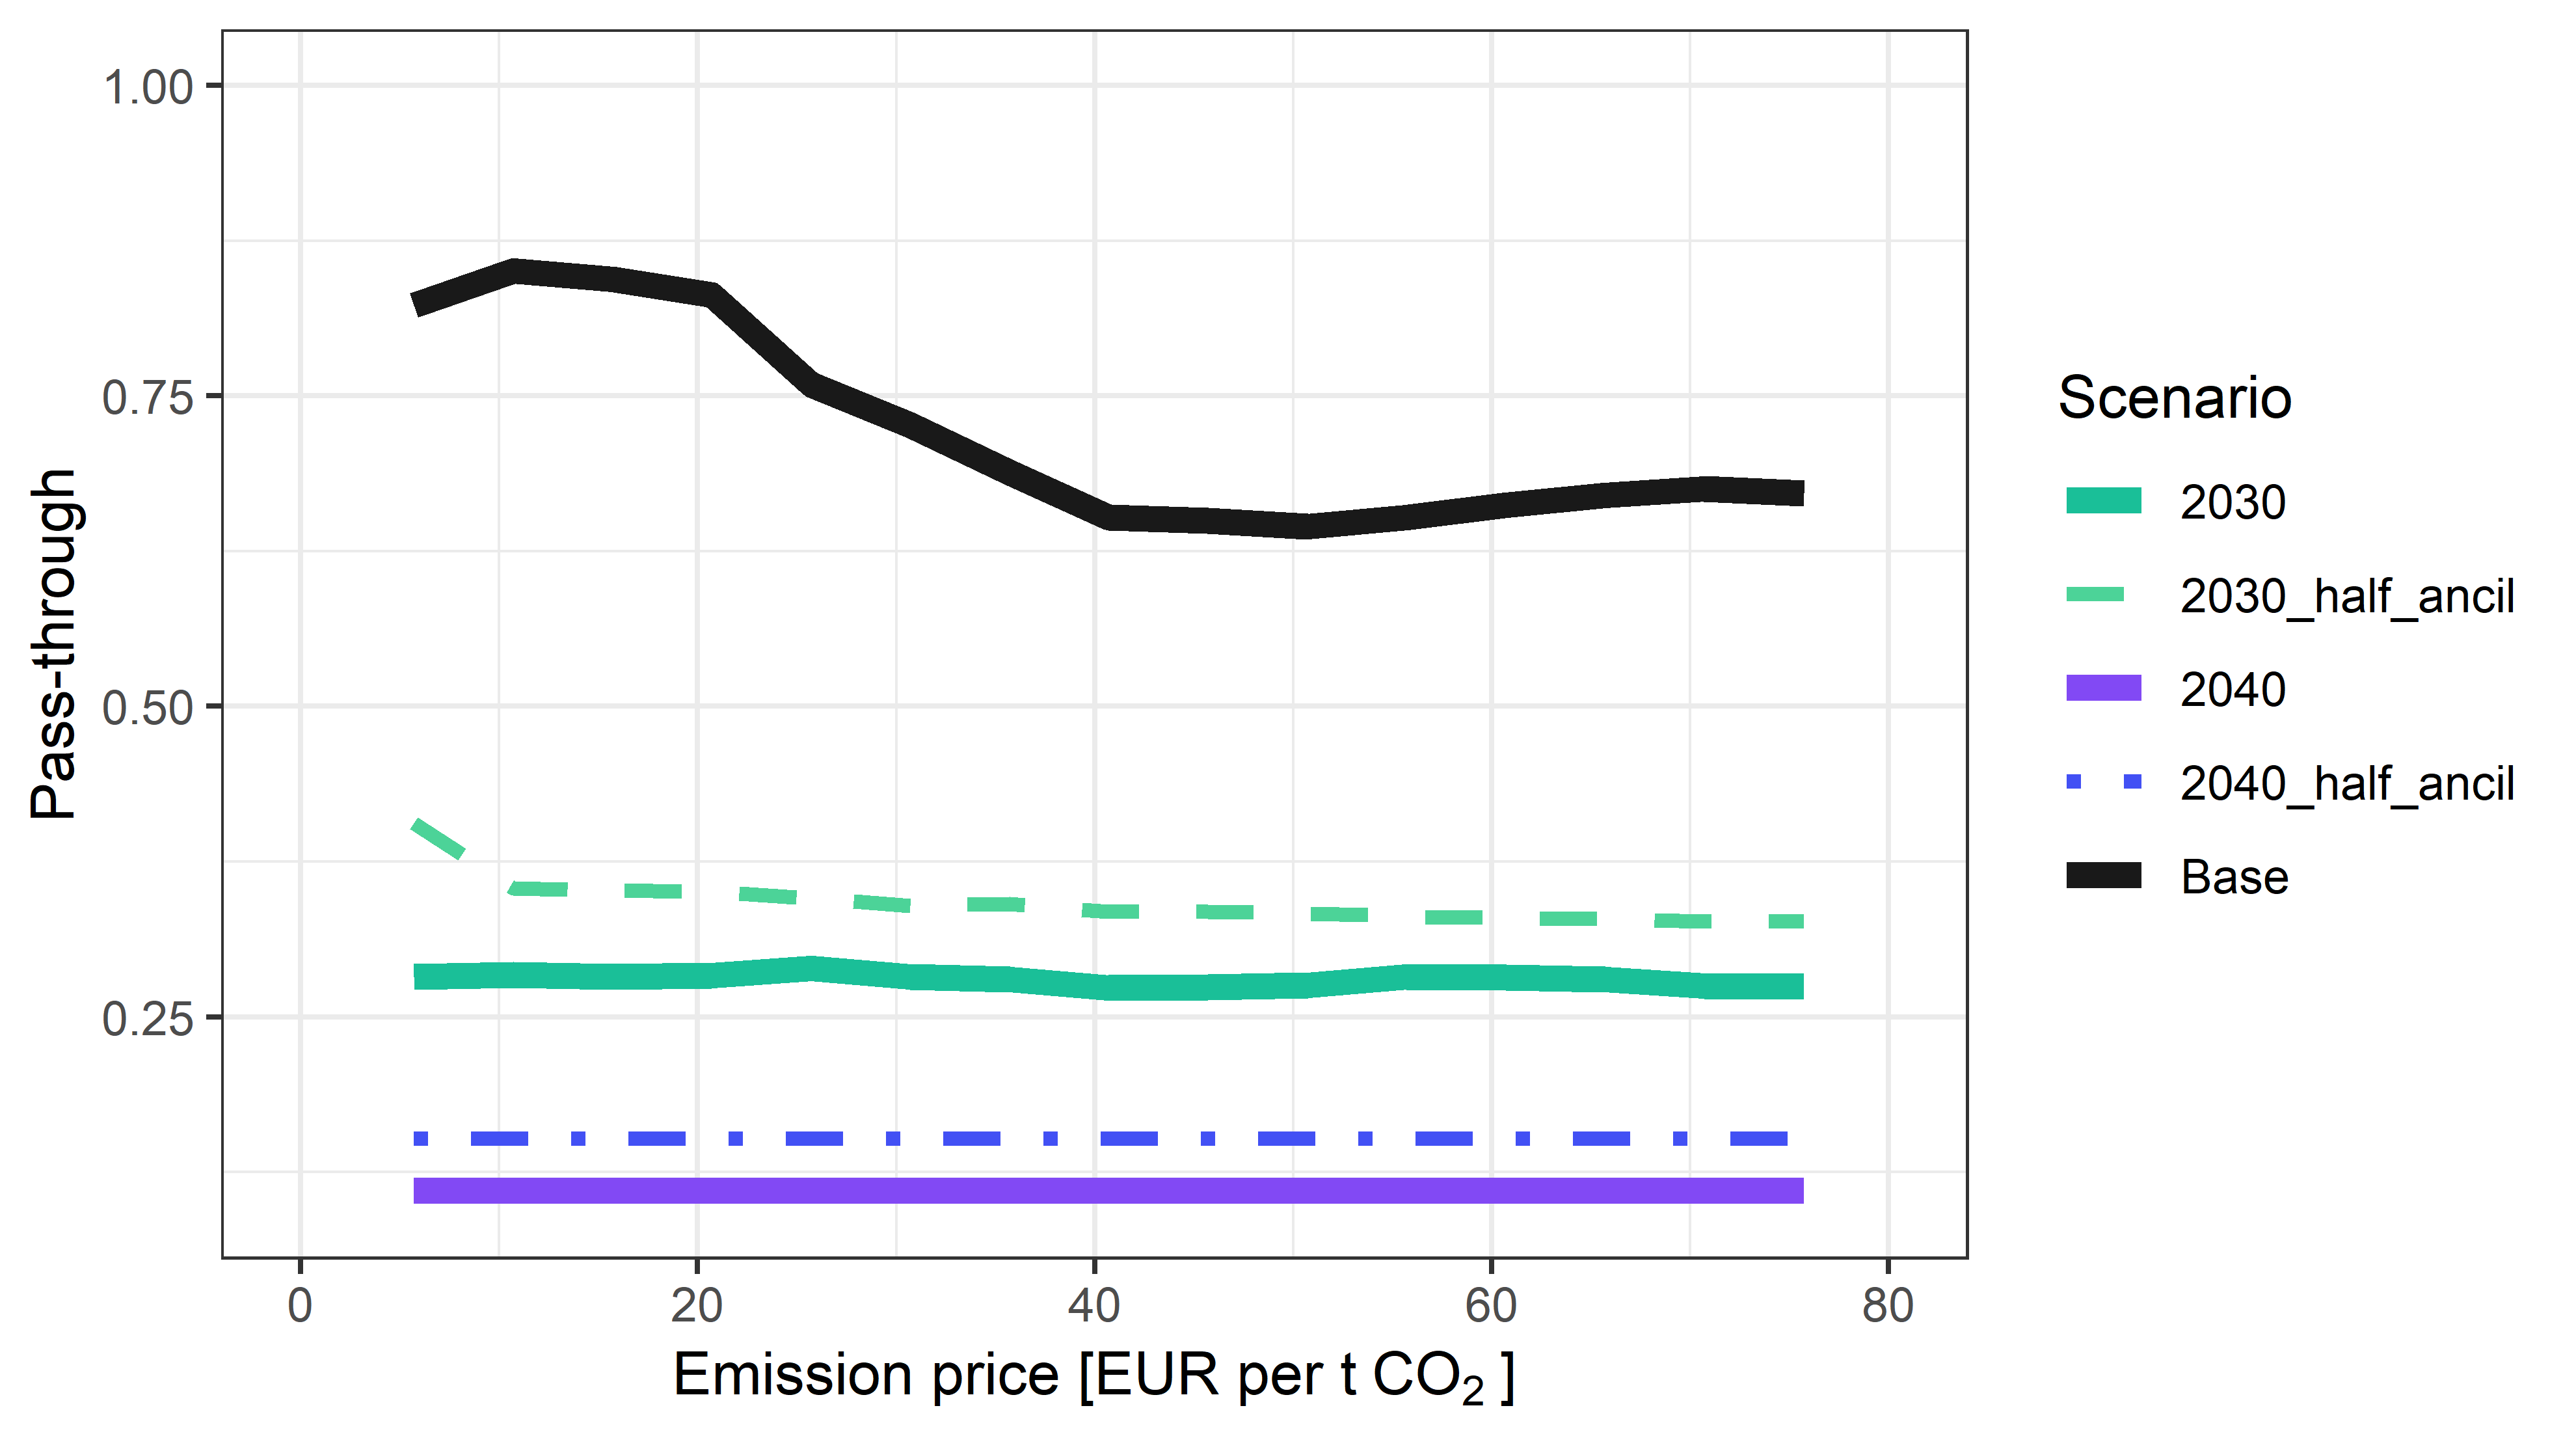
\includegraphics[scale=0.75]{Figure3d_future_sensitivity.png}
\caption{Pass-through estimates for future scenarios}\label{Fig3c}
\end{figure}
 
Given our assumptions for 2030, we estimate the carbon price pass-through at close to 0.28, with minor variation in response to the carbon price level. Due to the reduction of power generation capacities, substitution potential in response to rising carbon prices is firmly limited. Moreover, during most hours of the year the marginal unit is a low-emitting generator, reducing the carbon cost pass-through by between $0.57$ and $0.37$ compared to our baseline estimation for the year 2017. Increasing power system flexibility, modeled as halving the must-run capacity, has the potential to increase the pass-through level by $0.06$ on average. 
By 2040, in the absence of power generation from coal or lignite, emission cost pass-through declines to $0.11$ for all considered carbon prices as power generation is dominated by intermittent renewables, while low-emitting natural gas-fired generators are marginal infrequently.
Under these conditions, halving must-run capacity is not sufficient to raise the pass-through. Eliminating any must-run requirement leads to an average increase of $0.04$ in the emission cost pass-through. 

\section{Discussion} \label{sec_discuss}
Our estimates of emission cost pass-through in the current German electricity system are well in line with findings from econometric \citep{Hintermann2016} and model-based \citep{Lise2010} assessments of carbon-price pass-through in the literature. This is remarkable, as in contrast to some previous studies, our analysis features high (hourly) temporal  resolution to realistically incorporate power generation from intermittent renewable sources and endogenizes the price elasticity of electricity supply.
Yet, our results are valid only for the specific electricity systems that we studied and rest on several simplifying assumptions, most notably perfect competition on electricity wholesale markets and perfectly price-inelastic electricity demand. 

\begin{table}[h!]
\caption{Cost pass-through estimates for Germany based on COMPETES}
\smallskip
\centering
\begin{tabular}{l c c c c c}
\hline
\makecell{Market\\structure} & \makecell{Price elasticity\\of demand} & \makecell{Change in\\ \ce{CO2} cost} & \makecell{Chen et al.\\(2008)} & \makecell{Lise et al.\\(2010)} \\ \hline \hline
\makecell{perfect\\competition} & $0$ & $10$ & $0.92$ & -- \\ \hline
\makecell{perfect\\competition} & $0$ & $20$ & $1.18$ & $0.87$ \\ \hline
\makecell{perfect\\competition} & $0.2$ & $20$ & $0.8$ & $0.75$ \\ \hline
\makecell{oligopolistic} & $0.2$ & $20$ & $0.69$\footnote{Assuming EDF excercises market power in France} & $0.76$  \\ \hline

\makecell{perfect\\competition} & $0$ & $40$ & -- & $0.89$ \\ \hline
\makecell{perfect\\competition} & $0.2$ & $40$ & -- & $0.77$ \\ \hline
\makecell{oligopolistic} & $0.2$ & $40$ & -- & $0.65$ \\ \hline
\end{tabular}
\label{competes_results}
\end{table}

As \citet{Chen2008} and \citet{Lise2010} demonstrate, both assumptions can have significant effect on the estimated pass-through. 
For further illustration, Table \ref{competes_results} summarizes pass-through estimates from these publications employing the numerical model COMPETES to asses emission cost pass-through in imperfectly competitive European electricity markets.\footnote{Please note that reported pass-through estimates are not directly comparable to ours, as (marginal) emission cost pass-through is approximated for a change in emission cost from $0$~\euro{}/t\ce{CO2} to the level indicated as 'Change in \ce{CO2} cost'.}

Assuming the price elasticity of demand is $0.2$ instead of $0$ reduces the pass-through by approximately $0.12$. Likewise, going from perfect competition to oligopolistic competition can reduce pass-through by up to $0.12$ \citep{Lise2010}.
While the magnitude of the effect is potentially significant, one also needs to take into account how realistic these deviations from our assumptions are, when assessing our results. 

The German \citet{MPK2017}, which monitors the electricity market and advises the government on competition policy and regulation, finds no significant evidence of excessive market power on the German power market. 
% This is also acknowledged by \citet{XX}, who state “”.
Moreover, the short‐run price elasticity of electricity demand is empirically found to be very low \citep{Lijesen2007}. 
This suggests, that the estimation bias caused by assuming perfectly competitive markets and inelastic demand is likely small.
Likewise, moderate changes in net imports should not alter pass-through substantially, as our analysis in section \ref{robustn} suggests very limited sensitivity of carbon price pass-through to net electricity imports.
However, we only changed the magnitude of net imports but not the pattern of (net) imports over time. Hence, our analysis might not reveal the full impact of changes in the pan-European power plant dispatch on the emission cost pass-through caused by rising \ce{CO2} emission prices.
More frequent electricity imports from low-carbon sources (e.g. French nuclear power plants) could crowd out some of the \ce{CO2} emission intense production with high marginal emission cost.
This would reduce pass-through rates.
If, on the other hand, exports would increase in response to rising \ce{CO2} prices, pass-through rates could turn out to be higher than estimated.
Similarly, changes in the relative prices of coal and natural gas have little effect on carbon price pass-through at high levels of \ce{CO2} prices. Yet, at lower carbon prices, shifts in relative coal prices affect the pattern of power plant substitution, compressing or stretching the pass-through curvature, without systematically reducing cost pass-through. 
Further potential bias stems from the assumption of perfect substitutability of coal and natural gas in district heat generation. Requiring more emission intense heat generation than dispatched by our model would lower pass-through estimates , as the inflexibility works much like must-run constraints.

\section{Conclusions} \label{sec_conclude}
We have shown that emission cost pass-through to electricity prices is an important determinant of the current and even more so the future profitability of district heating systems. Moreover, emission cost pass-through with heterogeneous suppliers, such as in the electricity system, is affected by a wide variety of factors, including the emission price level itself.

Given our conservative estimation of technically required pass-through levels (see section \ref{CO2DHeffect}) and the small and likely upward-skewed bias in our estimates of system-wide pass-through, we currently see operators of district heating systems of moderate or better electrical efficiency ($\eta_{el}^{K} \geq 0.375$) in a position to benefit from any \ce{CO2} price increase up to the highest considered level (provided that boilers generate less than $20\%$ of total fossil heat generation)\footnote{As boilers are typically used for peak generation, this should hold for many, if not most DHC systems.}.
However, the long-run transition towards a decarbonized, highly renewable electricity system is a substantial challenge for DHSO profitability, in particular if the renewables expansion is accompanied by rising \ce{CO2} emission prices.
By 2030, even the most efficient CHP plants will no longer benefit from high emission prices, as the still remaining coal and lignite fired power plants will be inframarginal throughout most of the year. Increasing power system flexibility, which we modeled as a reduction in must-run capacity, could raise emission cost pass-through somewhat. Yet, at pass-through levels below $0.3$ profitability will still deteriorate even for the most efficient natural gas-fueled CHP plants. 
With the complete phase-out of coal, that the ‘coal commission’ dates to the late 2030s, emission prices will have little effect on electricity prices. In the face of high emission prices, DHSOs will then either have to pass on increasing costs to final heat prices or seek for other, low-emission heat generation options.

From the perspective of an owner of a natural gas-fired district heating system, an immediate increase in emission prices could be attractive, as the resulting 'windfall profits' could be invested in low-emission heat generation technologies. 
This would relieve such an DHSO from the pressure of high carbon prices that will intensify over time. 
However, this window of opportunity for DHSOs is closing at the speed of the coal exit.

Policy makers need to reconsider whether conventional district heating systems, which source their heat largely as a by-product from fossil power generation, are indeed a promising component of future energy systems. The current German target of $120$ TWh of heat generated by co-generation in 2025 \citep{KWKG2016} is likely to lock DHSOs into a generation structure built on fossil fuels that undermines DHSO profits, raises heat costs and falls short of potential carbon emission reductions.
\section*{Acknowledgements}
We gratefully acknowledge support from the European Research Council (“reFUEL" ERC-2017-STG 758149).

\newpage
\bibliographystyle{elsarticle-harv}
\bibliography{passtru_main}

\newpage
\appendix
\nocitesec{*}
\section{Description of the power system Model \emph{MEDEA}} \label{sec_datref} \label{Apndx2}
\subsection{Overview}
We use a simple, stylized and parsimonious model of the German and Austrian power system to estimate the pass-through from emission prices to electricity prices in the common bidding area.
Our power system model determines the cost-minimizing hourly dispatch of thermal and hydro storage power plants that is required to meet price-inelastic (residual) demand for electricity and district heat.
In total, $552$ thermal power plants and $62$ hydro storage plants are grouped in $34$ technology clusters. We differentiate the clusters by generation technologies (e.g. steam turbine, combustion turbine, combined cycle, etc.) and by fuels (uranium, lignite, hard coal, natural gas, mineral oil, biomass, water).
Thermal power plants burn fuels to generate electricity and are constrained in their operation by installed capacities for heat and power generation.
Heat generation is possible in heat boilers (aggregate capacity $30$ GWth, efficiency $0.9$) or in combined heat and power (CHP) plants, which must respect the limits of their feasible operation region.\footnote{The feasible operation region specifies all viable combinations of heat and power generation along with the required fuel use.}
Heat generation and consumption are aggregated, i.e. heat generators are not serving specific district heating systems.
Electricity generation from intermittent renewable sources (wind, solar, run-of-river) is given exogenously but can be curtailed.
Electricity can also be stored in reservoir and pumped hydro storages.
Generation from hydro storage plants is constrained by turbine capacity and energy contained in reservoirs of limited size.
Reservoirs are filled by inflows or by pumping (pumped storages only).
To better capture operational differences, we model daily, weekly and seasonal reservoir and pumped storage plants separately.
Electricity exchange with countries outside Austria and Germany is held fixed at hourly quantities realized in 2017.
To ensure a stable and secure operation of the electricity system, power plants must provide ancillary services such as frequency control or voltage support.
We assume that this requires generators with an installed capacity of at least $21$ GW\footnote{This is equal to 12.5\% of peak load plus 7.5\% of installed solar and wind power capacity and is broadly in line with findings by \citet{Hirth2015} and \citet{Nicolosi2012}.} to be operational (either generating or pumping in case of pumped hydro storages) at any point in time.
For a mathematical description see \ref{Apndx2}. The model is implemented in GAMS and was solved by Gurobi on an Intel Xeon Gold $6144$ with $264$ GB RAM.
%The model code can be found at \url{https://github.com/sebwehrle/medea}.

\subsection{Mathematical Description}
\subsubsection{List of Sets}
\begin{tabular}{c l}
$f \in F$ & fuels \\
$g \in G$ & generators \\
$CHP \in G$ & combined heat and power generators \\
$PSP \in G$ & hydro storage generators \\
$l \in L$ & limits to the feasible operation region of CHP plants \\
$p \in P$ & products generated \\
$t \in T$ & time periods (hours)
\end{tabular}

\subsubsection{List of Parameters}
\begin{tabular}{c l}
$\underline{a}$ & \makecell[l]{minimum generation level required for provision of \\ancillary services [MW]} \\
$\overline{C}_{g,p}$ & \makecell[l]{maximal generation of product $p$ by generator in \\cluster $g$ [MW]} \\
$\overline{STOR}_{g}$ & \makecell[l]{reservor storage capacity of hydro storage plant $g$ [MWh]} \\
$D_{t,p}$ & demand for product $p$ at time $t$ [MW] \\
$N_{g}$ & number of plants in cluster $g$ \\
$om_g$  & \makecell[l]{variable operation and maintenance cost of \\generator $g$ [\euro/MWh]} \\
$ORF_{g,l,f}$ & \makecell[l]{use of fuel $f$ at limit $l$ of the operating region of a \\CHP unit in cluster $g$ [MWh]} \\
$ORP_{g,l,p}$ & \makecell[l]{generation of product $p$ at limit $l$ of the operating \\region of a CHP unit in cluster $g$ [MWh]} \\
$P_{t,eua}$ & price of \ce{CO2} emissions at time $t$ [\euro/t~\ce{CO2}e] \\
$P_{t,f}$ & price of fuel $f$ at time $t$ [\euro/MWh] \\
$Q_{t,pv}$ & solar energy generated at time $t$ [MW] \\
$Q_{t,ror}$ & energy generated by run-of-river plants at time $t$ [MW]\\
$Q_{t,we}$ & wind energy generated at time $t$ [MW]\\
$Q_{t,nip}$ & net imports at time $t$ [MWh] \\
$Q_{t,res}$ & inflows into hydro reservoirs at time $t$ [MWh/h]\\
$em_{f}$ & emission factor of fuel $f$ [t \ce{CO2}/MWh fuel used]\\
$\eta_{g,f,p}$ & \makecell[l]{efficiency of generator $g$ using fuel $f$ to generate product $p$}\\

\end{tabular}

\subsubsection{List of Variables}
\begin{tabular}{c l}
$ppsp_{t,g}$ & \makecell[l]{energy pumped into pumped storage reservoirs at \\time $t$ [MWh]} \\
$qf_{t,g,f}$ & quantity of fuel $f$ used by generator $g$ at time $t$ [MWh]\\
$qp_{t,g,p}$ & energy generated by generator $g$ at time $t$ [MWh]\\
$qpsp_{t,g}$ & power generated by hydro storage plant $g$ at time $t$ [MWh]\\
$sconv_{t,g,l}$ & convexity variable $g$\\
$qstor_{t,g}$ & \makecell[l]{quantity of energy stored in hydro storage plant $g$ at \\time $t$ [MWh]}\\
$qns_{t,p}$ & non-served load of product $p$ at time $t$ [MWh]\\
$qct_{t}$ & quantity of energy curtailed at time $t$ [MWh]\\
\end{tabular}

\subsubsection{Mathematical model}
Our power system model uses a linear programming formulation of the economic dispatch problem for thermal units within the Austro-German bidding zone. Operation of pumped storage plants is also formulated as a linear problem.
The model's objective is to minimize total system cost, the sum of fuel, emission and operation and maintenance cost along with the cost associated with curtailment of renewable energies and loss of load.
\begin{align}
\min \left(\sum_{t,g,f}\left(\left(P_{t,f} + em_{f} P_{t,eua}+om_{g}\right) qf_{t,g,f} + qns_{t,p} M + qct_{t} N \right) \right)
\end{align}
In each hour the market has to clear, such that electricity supply from thermal and net generation from hydro storage plants plus power generation from non-dispatchable sources (wind energy, photovoltaics, and run-of-river hydro plants) equals electricity demand less net imports of electricity.
\begin{align}\label{12}
\begin{split}
D_{t,pwr} - Q_{t,nip} = \sum_{g} \left(q p_{t,g,pwr} \right) + \sum_{g\in PSP} \left(qpsp_{t,g} - ppsp_{t,g} \right) \\
+ Q_{t,we} + Q_{t,pv} + Q_{t,ror}, \forall t
\end{split}
\end{align}
In linear (economic dispatch) models, the marginals ('shadow prices') on equation (\ref{12}) can be interpreted as power prices in an energy-only market. We use these marginals to derive the pass-through from emission prices to power prices.
As we also consider co-generation of heat and power in our model, we introduce the heat balance equation (\ref{13}). Heat supply from CHP units and heat boilers must be adequate to meet district heating demand $D_{t,ht}$.
\begin{align}\label{13}
D_{t,ht} \leq \sum_{g \in CHP} \left( qp_{t,g,ht} \right) + qns_{t,p}, \forall t
\end{align}
Hourly generation of power and heat is constrained by installed capacity. 
\begin{align}
qp_{t,g,p} \leq \bar{C}_{g,p}, \forall t
\end{align}
Coproduction of heat and power in CHP-plants is governed by
\begin{align}
\sum_{l} sconv_{t,g,l} = 1, \forall g \in CHP \\
\sum_{l} sconv_{t,g,l} ORP_{g,l,p} = qp_{t,g,p}, \forall g \in CHP \\
\sum_{l} sconv_{t,g,l} ORF_{g,l,f} \leq qfuel_{t,g,f}
\end{align}
Power production by power-only generators is modelled as a linear function of plant efficiency
\begin{align}
qp_{t,g,pwr} \leq \sum_{f} \eta_{g,f,pwr} qf_{t,g,f}, \forall t, g \notin CHP  
\end{align}
Ancillary services must be provided by operating thermal generation units or active hydro storage plants (regardless of whether they are pumping or turbining).
\begin{align}
\underline{a} \leq qp_{t,g,pwr} + qpsp_{h,g} + qstor_{t,g}, \forall t
\end{align}
Operation of pumped storage plants is subject to the equations
\begin{align}
qpsp_{h,g} \eta_{g} \leq \overline{C}_{g}, \forall t, g \in PSP \\
ppsp_{t,g} \leq \overline{C}_{g}, \forall t, g \in PSP \\
qstor_{t,g} - qstor_{t-1, g} = ppsp_{h,g} \eta_{g} - qpsp_{h,g} \\
qstor_{t,g} \leq \overline{STOR}_{g}, \forall t, g \in PSP
\end{align}

\subsection{Data}
Information regarding the power plant stock (generation capacities, technology, locations) in Germany are based on data provided by the Open Power System Data (OPSD) project \citep{OPSD2018a}.
Data on Austrian power plants was collected through own research and includes information from the regulatory body~\citep{EControl2003}, sector associations~\citep{OeEn2017}, operating companies, and water registers of federal authorities~\citep{LandVorarlberg2018, LandTirol2018}.
Hourly electricity generation from intermittent sources (solar PV, wind) and load in Austria and Germany is also sourced from \citet{OPSD2018b}. 
Further time series on international commercial electricity exchanges, the aggregate filling rate of hydro reservoirs and storage plants, and the actual electricity generation and consumption of hydro power plants (including run-of-river plants) are obtained from ENTSO-E's transparency platform~\citep{ENTSOE2018}.
We approximate inflows of water to reservoirs in Austria by combining downsampled data on weekly water reservoir levels with hourly electricity generation and pumping from hydro reservoirs and pumped storage plants.\footnote{In Germany, 98\% of the installed hydro storage capacity is pumped hydro power so that we abstract from inflows to German hydro storage plants.}
Hourly district heating demand is estimated based on synthetic load profiles for natural gas demand~\citep{Almbauer2009}.
These load profile make use of daily average temperatures from MERRA-2 satellite data~\citep{GMAO2015} and are scaled to total final consumption of district heat in Germany and Austria.\footnote{As final data for the consumption of district heat in 2017 was not published at the time of writing, we scale 2016 district heat consumption by the relative change in heating degree days from 2016 to 2017~\citep{AGEB2018a, OeStat2018}.}
Realized prices of hard coal, natural gas and EU emission allowances for the year 2017 are taken from the \citet{EEX2019}.
Prices for mineral oil are approximated on the basis of prices for Brent crude oil as published by the~\citet{EIA2018}.
As there are no market prices for nuclear fuel and lignite, we estimate lignite cost at $5.50$~\euro{}/MWh (including mining, but excluding emission cost) and $3.50$~\euro{}/MWh for nuclear fuel.
Descriptive Statistics for all used time series are displayed in Table~\ref{Tab2}.

\begin{table}[t!]
\caption{Descriptive statistics}
\smallskip
\centering
\begin{tabular}{c c c c c c c}
\hline
 & Unit & Min & Max & Mean & Std. Dev & Source \\ \hline \hline
Wind & $GW$ & $0.279$ & $41.72$ & $12.49$ & $9.03$ & OPSD \\ \hline
Solar PV & $GW$ & $0$ & $28.33$ & $4.23$ & $6.49$ & OPSD \\ \hline
Run-of-river & $GW$ & $2.08$ & $7.13$ & $4.78$ & $1.13$ & ENTSO-E \\ \hline
\makecell{Reservoir \\ inflows} & $GW$ & $0$ & $2.14$ & $0.79$ & $0.59$ & \makecell{own\\ calculations} \\ \hline
\makecell{Electricity \\consumption} & $GW$ & $38.52$ & $96.77$ & $69.09$ & $12.59$ & ENTSO-E \\ \hline
\makecell{District heat \\ consumption} & $GW$ & $1.54$ & $42.04$ & $13.49$ & $9.60$ & \makecell{own \\calculations} \\ \hline
\makecell{Net imports \\ (commercial \\exchange)} & $GW$ & $-13.74$ & $7.07$ & $-4.87$ & $2.93$ & ENTSO-E\\ \hline
\makecell{Coal price \\(API2)} & \euro{}$/MWh_{th}$ & $8.32$ & $11.36$ & $9.65$ & $0.72$ & eex \\ \hline
\makecell{Natural gas \\price (NCG)} & \euro{}$/MWh_{th}$ & $15.91$ & $19.02$ & $17.27$ & $0.87$ & eex\\ \hline
\makecell{Mineral oil \\price} & \euro{}$/MWh_{th}$ & $23.18$ & $32.93$ & $28.25$ & $2.57$ & EIA\\ \hline
\makecell{EU Emission \\Allowance price} & \euro{}$/MWh_{th}$ & $4.41$ & $8.21$ & $5.89$ & $1.11$ & eex\\
\hline \hline
\end{tabular}
\label{Tab2}
\end{table}

\subsection{Model calibration and goodness-of-fit}
\begin{figure}[t]
\centering
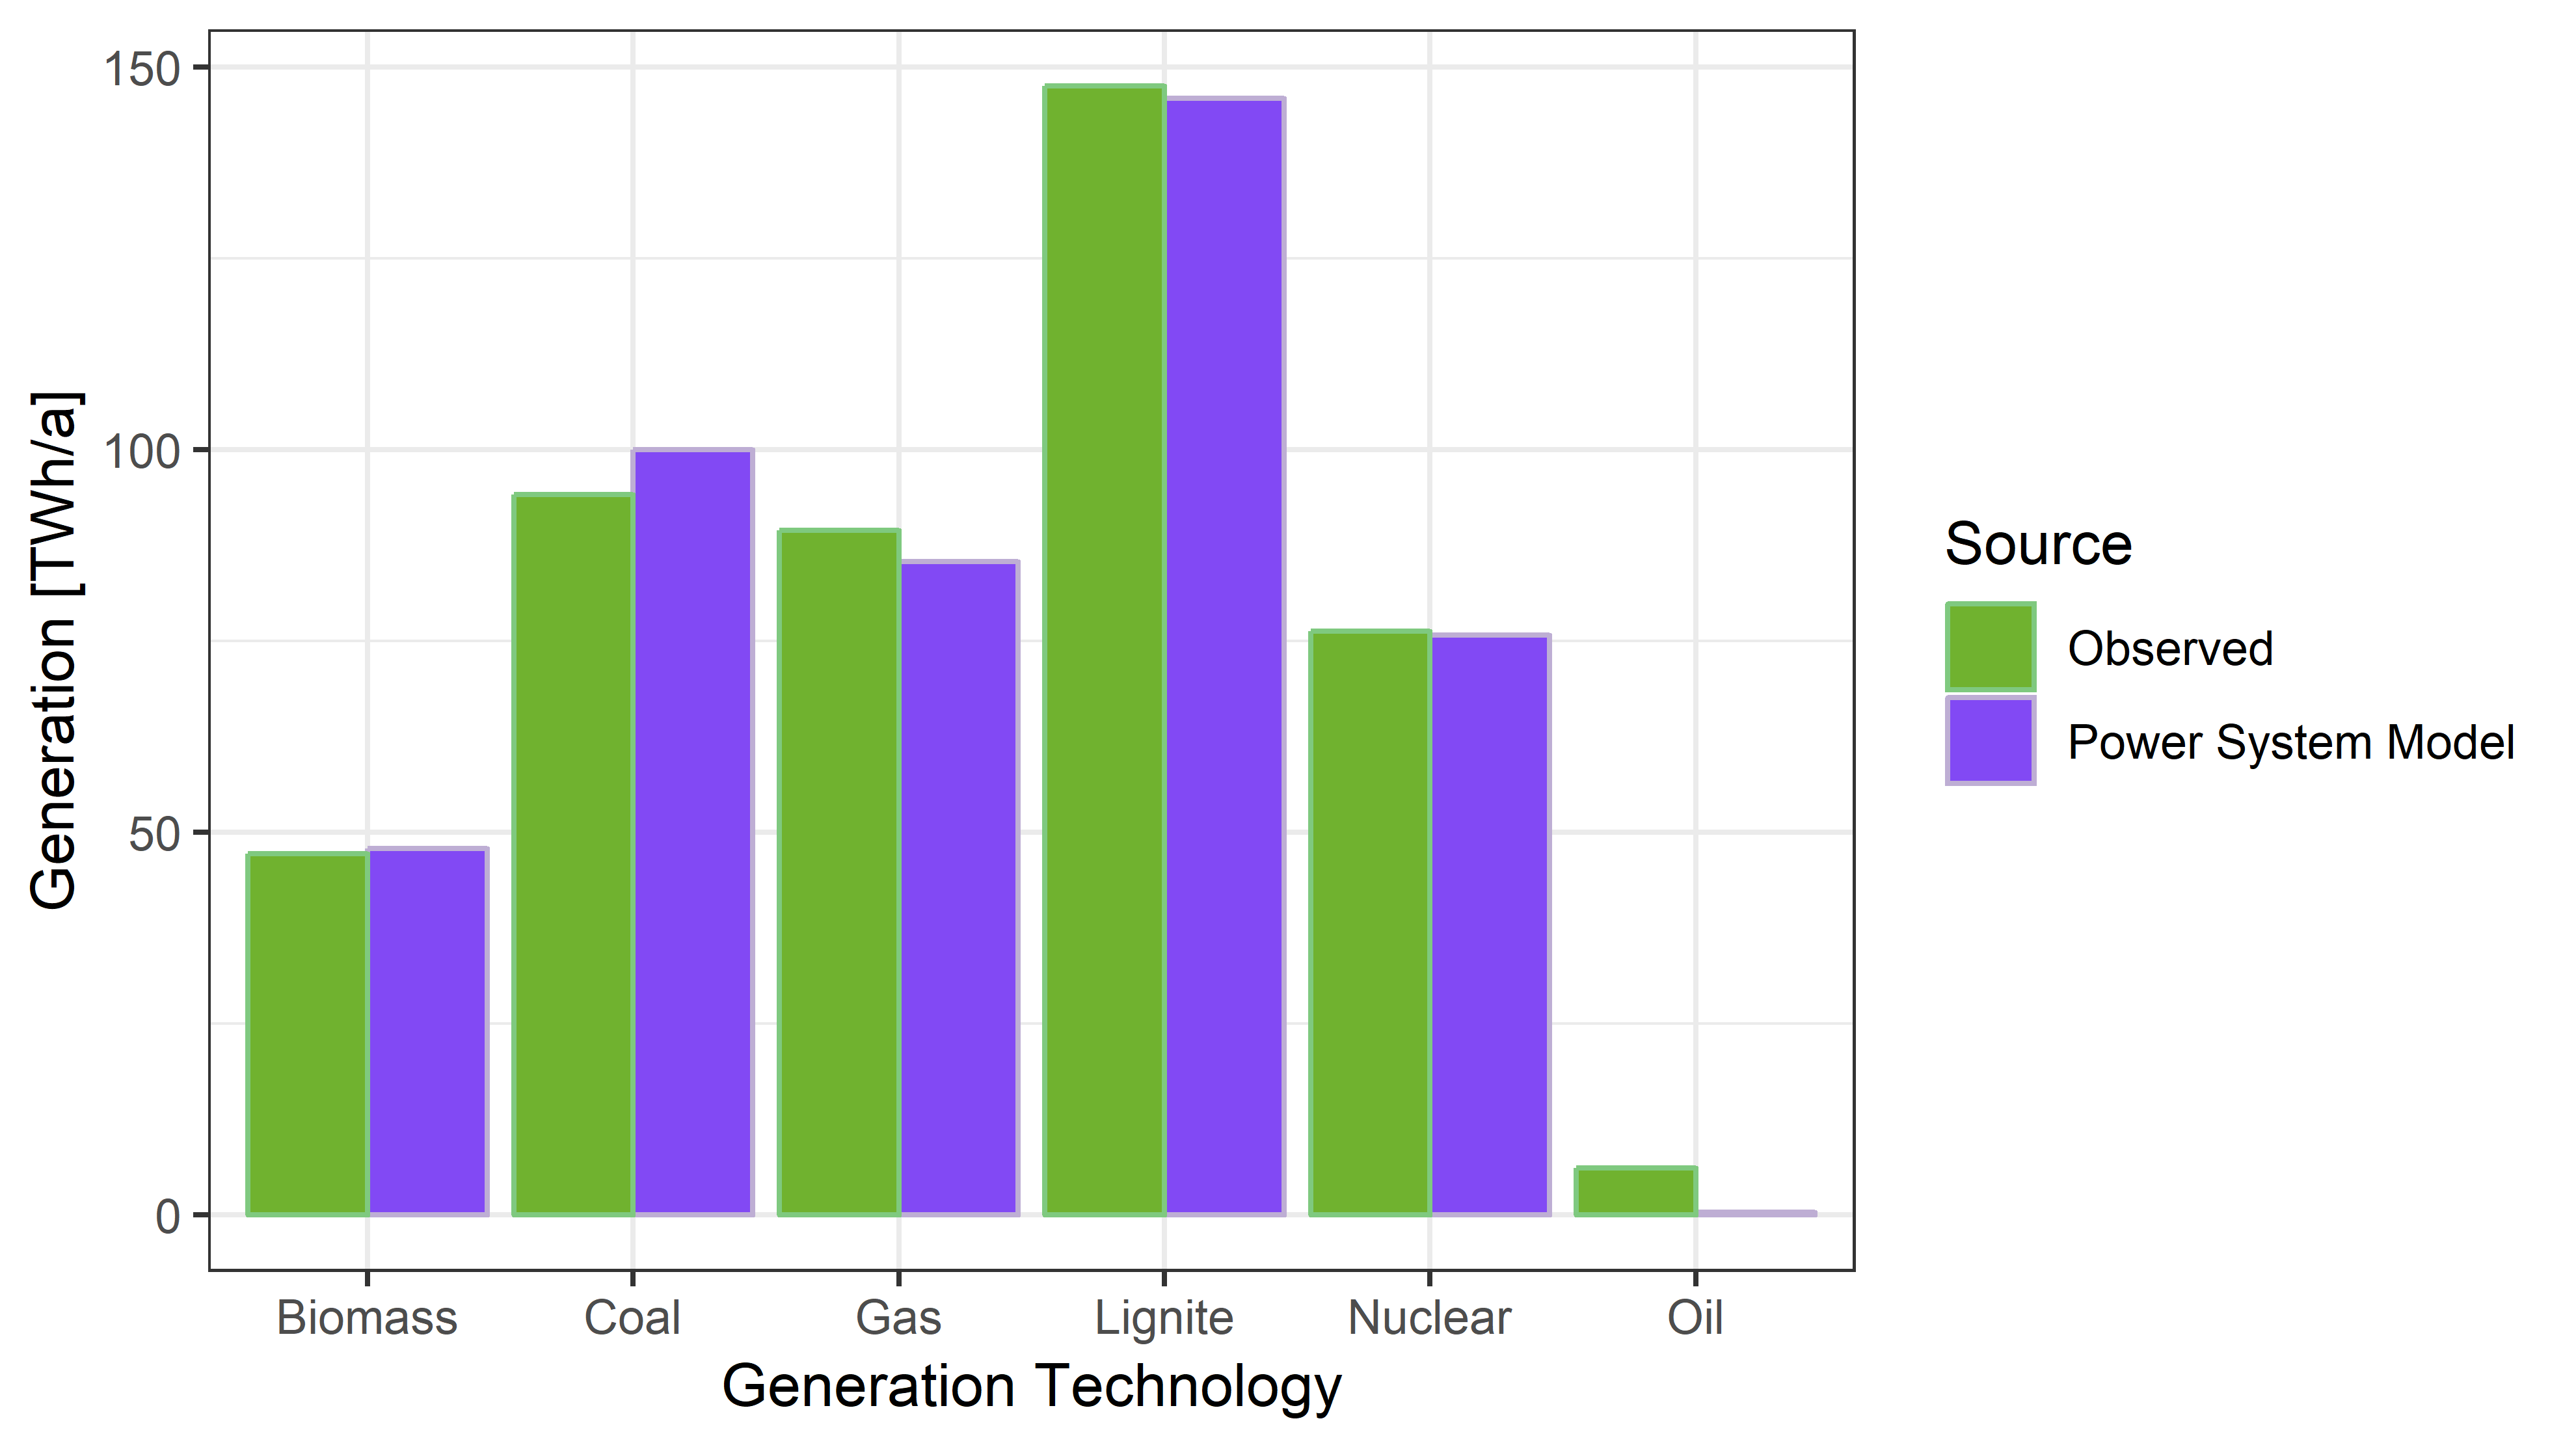
\includegraphics[scale=0.75]{Figure2_calibration.png}
\caption{Actual and model derived fuel burn (2017)}\label{Fig2}
\end{figure}

We use power plant efficiencies and availabilities to calibrate our power system model on actual data for quantities of fuel burnt for power generation~\citep{AGEB2018, OeStat2018} and greenhouse gas emissions \citep{UBA_DE2018a, UBA_DE2018b} from 2017.
\footnote{For Austria, the most recent data on GHG emissions and fuel burn for power generation available at the time of writing relates to 2016. As Austria’s electricity consumption is only around one tenth of Germany’s and roughly two-third of power generation in Austria stems from hydro power plants, the induced error should, however, be small.} 

As visible in figure \ref{Fig2}, our model is able to replicate fuel burn and emissions fairly well, although the use of coal is somewhat overstated ($+5.9$ TWh), while consumption of natural gas and oil are underestimated by $4.0$ TWh and $5.7$ TWh. Overall, modelled \ce{CO2} emissions from power generation of $316.4$ million tonnes are falling short of near time estimates by around $2.4\%$ or $7.9$ million tonnes.
Comparing the model-derived hourly shadow prices of electricity to actual day-ahead prices at the European Energy Exchange in 2017, we observe a correlation of $0.80$ and a root mean squared error (RMSE) of $10.91$.

\bibliographystylesec{elsarticle-harv}
\bibliographysec{passtru_appendix}

\end{document}
